
% --------------------------------------------------------------------
% LaTeX2e - Modifizierter Rahmen fuer 
% Ausarbeitungen basierend auf
% dem Muster von M. Haag (27.09.1995) 
% durch J�rgen Graf (irgendwann 2007)
% und Stephan Puls (Ende 2010)
% -------------------------------------------------------------------

\documentclass[12pt,twoside,a4paper]{report}
\usepackage{mysty,epic,eepic,bibdef,bibhyphen,german,makeidx,longtable,time,theorem,amsmath,amssymb,uhrzeit,multirow,ifpdf}
\usepackage[latin1]{inputenc}
\usepackage{url}
\usepackage{algorithm, algpseudocode}
\urlstyle{sf}

% ------------------------------------------------------------------
% Pakete in Zusammenhang mit pdflatex einbinden
% -------------------------------------------------------------------
%\newif\ifpdf
%\ifx\pdfoutput\undefined
%    \pdffalse           % we are not running PDFLaTeX
%\else
%    \pdfoutput=1        % we are running PDFLaTeX
%    \pdftrue
%\fi
%----------------------------------------------------------------------
\ifpdf
    \usepackage[pdftex,
        colorlinks=true,
        urlcolor=blue,                      % \href{...}{...}
        anchorcolor=rltbrightblue,
        filecolor=green,                    % \href*{...}
        linkcolor=black,                % \ref{...} and \pageref{...}
        menucolor=webdarkblue,
        citecolor=rltgreen,
        pdftitle={},
        % TODO: Hier Deinen Namen eintragen
        pdfauthor={Dein Name},
        pdfsubject={},
        pdfkeywords={},
        pagebackref=true,
        %pdfpagemode=None,
        bookmarksopen=true]{hyperref}
    \pdfcompresslevel=9
    \usepackage[pdftex]{graphicx}
    \usepackage{thumbpdf}
\else
    \usepackage[
        colorlinks=true,
        urlcolor=black,                 % \href{...}{...}
        anchorcolor=black,
        filecolor=black,                    % \href*{...}
        linkcolor=black,                % \ref{...} and \pageref{...}
        menucolor=black,
    pagebackref=true,
        citecolor=black]{hyperref}
    \usepackage{graphicx}
\fi
 \usepackage{color}
\definecolor{rltbrightred}{rgb}{1,0,0}
\definecolor{rltred}{rgb}{0.75,0,0}
\definecolor{rltdarkred}{rgb}{0.5,0,0}
%
\definecolor{rltbrightgreen}{rgb}{0,0.75,0}
\definecolor{rltgreen}{rgb}{0,0.5,0}
\definecolor{rltdarkgreen}{rgb}{0,0.25,0}
%
\definecolor{rltbrightblue}{rgb}{0,0,1}
\definecolor{rltblue}{rgb}{0,0,0.75}
\definecolor{rltdarkblue}{rgb}{0,0,0.5}
%
\definecolor{webred}{rgb}{0.5,.25,0}
\definecolor{webdarkblue}{rgb}{0,0,0.75}
\definecolor{webbrightgreen}{rgb}{0,0.5,0}


%  Use alternative backref in newer versions of backref and
%  redefine the backreference. You can redefine \backrefalt
%  to suit your requirements.

   \newcounter{countCites}
   \newcounter{countNotCited}
   \backrefgerman
   \renewcommand*{\backref}[1]{}
   \newcommand{\backreftext}[1]{\footnotesize{\textsf{#1}}}

   \renewcommand*{\backrefalt}[4]{%
      \ifcase #1 %
          \backreftext{\textcolor{green}{\textbf{(NICHT ZITIERT)}}}%
      \stepcounter{countNotCited}
          \stepcounter{countCites}
      \or
         \backreftext{(Zitiert auf Seite~#2)}%
     \stepcounter{countCites}
      \else
         \backreftext{(Zitiert auf Seiten~#2)}%
     \stepcounter{countCites}
      \fi}




% -------------------------------------------------------------------
% Index erstellen (optional)
% -------------------------------------------------------------------
%\makeindex


%Grafiken ausblenden:
%\makeatletter
%  \renewcommand{\Ginclude@eps}[1]{}
%\makeatother

%Text ausblenden I:
%\usepackage{color}
%\color{white}


% -------------------------------------------------------------------
% globale Layout-Einstellungen:
% -------------------------------------------------------------------

\renewcommand\textfraction{0.0}
\renewcommand\bottomfraction{1.0}
\renewcommand\topfraction{1.0}
\renewcommand\arraystretch{1.2} %spacing between rows
\renewcommand{\baselinestretch}{1.0} % Zeilenabstand

% eigene Anpassungen (bei Bedarf):
% \input{my_commands}

\renewcommand\textfraction{0.15}
\addtolength\intextsep{5mm}
\addtolength\floatsep{5mm}
\addtolength\textfloatsep{5mm}

% Ende der eigenen Anpassungen

\global\parindent=0pt % 5pt
\global\parskip=1.5\smallskipamount\relax

\marginparsep 0.0cm
\textheight 22cm
\textwidth 15.5cm
\oddsidemargin 0cm
\evensidemargin 0cm

\setcounter{tocdepth}{3}
\setcounter{secnumdepth}{3}

\setlength{\unitlength}{1mm}

% ---- globale Definitionen
% evtl. in eigene Datei
%\input{Definitionen}

% ===================================================================
% Makros (J�rgen Graf, 07.06.2006)
% ===================================================================
\theoremstyle{plain}
\newtheorem{definition}{Definition}[chapter]
\newtheorem{theorem}{Satz}[chapter]
\newtheorem{lemma}{Lemma}[chapter]
\newtheorem{proposition}{Proposition}[chapter]
\newtheorem{corollary}{Korollar}[chapter]
\newtheorem{observation}{Beobachtung}[chapter]
\newtheorem{fact}{Fakt}[chapter]
\newtheorem{procedure}{Prozedur}[chapter]
\newtheorem{postulat}{Postulat}[chapter]
%\newtheorem{proof}{Beweis}[chapter]
{\theorembodyfont{\rmfamily}
\newtheorem{remark}{Abschlie�ende Bemerkung}[subsection]
\newtheorem{example}{Beispiel}[chapter]
}

\newbox\ProofSym
\setbox\ProofSym=\hbox{
  \unitlength=0.18ex
  \begin{picture}(10,10)
    \put(0,0){\framebox(6,6){}}
%    \put(0,3){\framebox(6,6){}}
  \end{picture}
}

\newenvironment{proof}%
{\noindent{\em \iflanguage{german}{Beweis}{Proof}.\hspace{2mm}}}%
{\hfill\copy\ProofSym\linebreak}

% Abk�rzungen f�r die reellen, nat�rlichen, ganzen,... Zahlen
\newcommand{\R}{{\ensuremath{\mathbb{R}}}}
\newcommand{\N}{{\ensuremath{\mathbb{N}}}}
\newcommand{\Z}{{\ensuremath{\mathbb{Z}}}}
\newcommand{\C}{{\ensuremath{\mathbb{C}}}}
\newcommand{\Q}{{\ensuremath{\mathbb{Q}}}}
\newcommand{\F}{{\ensuremath{\mathbb{F}}}}
\newcommand{\Prim}{{\ensuremath{\mathbb{P}}}}

\newcommand{\mo}{\texttt{Motris}}
% ===================================================================
% BEGIN DOCUMENT
% ===================================================================
\begin{document}
% PDFLATEX-CHANGE
\ifpdf
    \DeclareGraphicsExtensions{.jpg,.png,.pdf}
\else
    \DeclareGraphicsExtensions{.eps,.ps}
\fi
% PDFLATEX-CHANGE

\pagestyle{empty}

% -------------------------------------------------------------------
% Titel:
% -------------------------------------------------------------------
% --------------------------------------------------------------------
% LaTeX2e - Rahmen fuer Diplomarbeiten; 27.09.1995 - M. Haag
% --------------------------------------------------------------------
% Aenderungen: M.Arens, 05.10.2001, Anpassung des Unilogos an pdflatex
% Aenderungen: J. Graf, 23.09.2010, Anpassung des Unilogos an pdflatex
% --------------------------------------------------------------------


% --------------------------------------------------------------------
% Titelseite:
% --------------------------------------------------------------------

%\input{unilogo}

\newcommand{\betreuerfont}{\large}
\newcommand{\iconunifont}{\bf}
\newcommand{\icontextfont}{\large}
\newcommand{\headerfont}{\huge \bf}
\newcommand{\authorfont}{\Large \bf}
\newcommand{\diplfont}{\Large \bf}

% --------------------------------------------------------------------
% Kopf:
% --------------------------------------------------------------------
\vfill
\vskip 2cm
\begin{center}
 \fbox{
  \begin{minipage}{14.5cm}
    \parbox{0cm}{\rule{0cm}{3.5cm}} % bestimmt Hoehe der fbox
    \hfill
    \parbox{4.5cm}{
\includegraphics[width=4.5cm]{Abbildungen/kit_logo_de_farbe_positiv}}
    \hfill
    \begin{minipage}{8.5cm}
        \icontextfont
        \baselineskip17pt
        \begin{center}
          {\iconunifont Karlsruher Institut\\f�r Technologie (KIT)} \\[3pt]
      { Institut f�r Prozessrechentechnik, } \\
      { Automation und Robotik (IPR) } \\
          der Fakult�t f�r Informatik
        \end{center}
    \end{minipage}
    \hfill
  \end{minipage}
 }
\end{center}
\vfill
% --------------------------------------------------------------------
% Titel:
% --------------------------------------------------------------------

\begin{center}
{
\headerfont
\baselineskip29pt

% TODO: Hier den Titel der Arbeit eintragen
Markerbasierte Objektverfolgung f�r die Mensch-Roboter-Kooperation



\vfill
\baselineskip20pt
\vskip 1 cm
%

\diplfont
% TODO: Hier den Typ der Arbeit w�hlen
%Praktikumsbericht\\
%Studienarbeit\\
Diplomarbeit\\
%Interner Bericht\\
%Seminararbeit\\
%Bachelorarbeit\\
%Masterarbeit\\
\authorfont
von\\

% TODO: Hier der Name des Autors eintragen
Beibei Cao \\
~\\

%\betreuerfont

%
}
%\end{center}
\vfill

% --------------------------------------------------------------------
% Betreuer:
% --------------------------------------------------------------------

%\begin{flushleft}
\betreuerfont
\baselineskip21pt
%\centerline{Stand: \today, \uhrii}
\centerline{Stand: \today}
\vspace{1cm}
% TODO: Hier den Titel und Namen des Betreuers eintragen
Referenten:
Prof. Dr.-Ing. Heinz W�rn \\
%\hspace{1,5cm}
Betreuer: Dipl.-Inform. Stephan Puls\\
%\end{flushleft}
\end{center}
\vfill

\cleardoublepage  % nur fuer die Endfassung

% -------------------------------------------------------------------
% Bemerkungen:
% hier kommen Anmerkungen rein, z.B. noch nicht verarbeitete
% Literaturhinweise
% -------------------------------------------------------------------
%\input{Bemerkungen}
%\cleardoublepage

% -------------------------------------------------------------------
% Erklaerung:
% (nur fuer die Endfassung)
% -------------------------------------------------------------------

%\input{Erklaerung}
%\cleardoublepage

% -------------------------------------------------------------------
% Danksagung:
% (optional, nur fuer die Endfassung)
% -------------------------------------------------------------------
%\input{Danksagung}
%\cleardoublepage

% -------------------------------------------------------------------
% Kurzfassung:
% -------------------------------------------------------------------
%\input{Kurzfassung}
%\cleardoublepage

% -------------------------------------------------------------------
% Verzeichnisse:
% -------------------------------------------------------------------

\pagestyle{headings}    % jetzt mit Seitennummern und Kopfzeilen
\pagenumbering{roman}   % aber Seitennummern mit roemischen Ziffern

\tableofcontents        % Inhaltsverzeichnis
\cleardoublepage

%\listoffigures          % Abbildungsverzeichnis
%\cleardoublepage

%\listoftables           % Tabellenverzeichnis
%\cleardoublepage

%\clearpage

% -------------------------------------------------------------------
% Hauptteil:
% -------------------------------------------------------------------

\pagenumbering{arabic}  % ab hier arabische Seitennummern, bei 1
                        % beginnend

% TODO: Ab hier die Kapitel einf�gen

% Zum Beispiel:
\chapter{Einleitung}

\section{Motivation}
Die St�rken von Robotern liegen in der Wiederholung von einfachen Handhabungst�tigkeiten. Dagegen sind Menschen mit ihren kognitiven F�higkeiten einzigartig, etwa in Bezug auf ihren Verst�ndnis der Aufgabe. Die Kombination von Mensch und Roboter kann Aufgaben stark rationalisieren, sofern jedem die optimalen Arbeitsteile zugewiesen wird. Die Anwendungsbereiche der Mensch-Roboter-Kooperation vergr��ern sich derzeit auf dem Feld der Medizin sowie der Industrie immer schneller. Damit Menschen und Roboter in einer geringen Entfernung sicher und effizient zusammenarbeiten k�nnen, ist die Erkennung bzw. die Verfolgung von Menschen und Objekten f�r ein Mensch-Roboter-Kooperation-System notwendig. Die Menschenerkennung garantiert die Sicherheit f�r den Menschen und liefert gleichzeitig Informationen �ber dessen Blickrichtung, um Aussagen �ber die Aufmerksamkeit des Menschen treffen zu k�nnen. Die Objekterkennung vereinfacht die Kommunikation zwischen Mensch und Roboter, wodurch die Fremdobjekte ohne weitere Programmierung direkt vom Roboter erkannt werden k�nnen. Au�erdem vermeidet die Objektverfolgung auch die Kollision zwischen Roboter und anderen Anlagenteilen.


\section{Aufgabenstellung}
Das Rahmenwerk MAROCO wird am Institut f�r Prozessrechentechnik, Automation und Robotik (IPR) entwickelt, damit Menschen und Roboter in einer gemeinsamen Umgebung sicher zusammenarbeiten k�nnen. Die Erfassung des Menschen und die Handlungsanalyse in der Szene erlauben es, die Gefahren von Roboterbewegungen f�r Menschen zu minimieren. Jedoch ist die Erkennung zurzeit auf das Menschmodell beschr�nkt. Alle anderen Objekte werden von dem System als Zylinder dargestellt. Das Ziel dieser Arbeit besteht darin, die verschiedenen Objekte zu kalibrieren und die entsprechenden geometrischen Charakteristika in dem System zu speichern, um dann die Objekte mit Hilfe der gespeicherten Informationen wiederzuerkennen und zu verfolgen. Beide Schritte sollen in Echtzeit durchgef�hrt werden.
\\
\\
%Eine spezielle auf Punktwolke basierte Methode werde f�r die Objektkalibrierung implementiert, die mithilfe der Pyramide die verschiedenen Objekte unterscheiden kann. Jedes Objekt wird als ein Graph mit Knoten und Kanten im System gespeichert. Im Teil der Objekterkennung bzw. Objektverfolgung wird ein Teilgraph-Tracker realisiert, was eine schnelle, stabile und pr�zise Spur liefern kann, obwohl einige Teile des Objekts verdeckt sind. Au�erdem ist die Stereo Korrespondenz als die Voraussetzung aller Funktionen sehr wichtig. Ein auf Singul�rwertzerlegung basiertes Matchingsverfahren wird f�r infrarot Bild implementiert. 


Folgende Ziele sollen erreicht werden:
\begin{itemize}
\item Objektsegmentierung,
\item Darstellung und Speichern des charakteristischen Modells der Objekte,
\item Objektwiedererkennung und Verfolgung,
\item Einhaltung der Echtzeitbedingungen (Framerate $\geq$ 30fps).
\end{itemize}

\chapter{Stand der Forschung}

3D Objekterkennung und Verfolgung kommt in vielen Anwendungsbereichen zum Einsatz. Daher wurden viele Algorithmen bzw. Systeme daf�r in den vergangenen Jahrzehnten entwickelt. Ein gutes Beispiel ist das kommerzielle Erkennungssystem von VICON \cite{VIC}. In dem System werden 8 Kameras benutzt, die von verschiedenen Richtungen das Zielobjekt bzw. Person beobachten. Einige wei�e Marken werden vorher am Ziel angebracht, damit seine Positionen und Bewegungen von den Kameras gut erkannt werden k�nnen. Nach Vergleichen der Bilder von verschiedenen Kameras kann ein 3D Modell des Ziels in Echtzeit erzeugt werden. Das System wird im Bereich von Computerspielen und Filmindustrie sehr oft benutzt. Ein anderes Beispiel ist das neue Ger�t Kinect von Microsoft XBox360 \cite{KIN}. Eine 3D Kamera kann die 3D Daten von Spielern ansammeln, damit die Spieler das Spiel direkt mit ihren K�rpern statt des traditionellen Kontroller steuern k�nnen. Die Analyseverfahren der Objekterkennung basieren auf unterschiedlichen Charakteristika der Objekte und sind f�r verschiedenen Typen von Objekten geeignet. In der Arbeit von Lepetit und Fua sind die aktuelle Verfolgungsverfahren in zwei gro�e Gruppen unterschieden worden: auf Marken basierte Objektverfolgungen und auf nat�rlichen Merkmale basierte Objektverfolgungen. Die Verfahren in der zweiten Gruppe k�nnen weiter in kantenbasiertes Verfahren, optischer Fluss basiertes Verfahren, Templatebasiertes Verfahren, Punktebasiertes Verfahren und das SLAM-Verfahren unterteilt werden \cite{LF05}. Im folgenden Abschnitt werden kurz die Details jedes Verfahrens erkl�ren.    

%In unserem System k�nnen alle Objekte in zwei Typen eingeteilt werden: die Objekte, die immer eine Seite zur Kamera richten, d.h. nur Bewegungen der Objekte in der Ebene von der Kamera beobachtet werden; und andere Objekte, die sich frei im Raum bewegen. Wir benennen den ersten Typ als feste Objekte z.B. der Arbeitsplatz, und den zweiten Typ als frei bewegte Objekte, z.B. das Werkzeug. Im Folgenden werden aktuelle Forschungsarbeiten �ber Objekterkennungsverfahren f�r beide Typen von Objekten erkl�ren.


%\section{Feste Objekte}
%Das Problem f�r die Erkennung der festen Objekte kann als die Objekterkennung mit planaren Marken zusammengefasst werden. In diesem Bereich sind viele Systeme f�r die Erweiterte Realit�t implementiert worden. 

\section{Standardmarkenbasierte Verfahren}
Die Verfolgungsverfahren k�nnen in zwei Schritte unterteilt werden: zuerst der Informationen von Bildsequenzen ansammeln um dann die Position des erkannten Objekts zu bestimmen. Die vordefinierte Marken k�nnen in beiden Schritten mehr Information liefern, damit die Objekte schneller und einfacher verfolgt werden k�nnen. Deshalb sind in diesem Bereich viele Systeme f�r die Erweiterte Realit�t implementiert worden. Ein Echtzeitsystem f�r Erweiterte Realit�t wurde von Zhang und Navab f�r Objektverfolgung in einer Industrieumgebung realisiert \cite{ZN00}. Sie haben eine Gruppe von 4 Vierecken als eine Marke benutzt. Die Marke wird durch Farbe und wei�e Flecken innerhalb der Vierecke kodiert. 
\\
\\
Ein anderes System hei�t ARToolKit, was vom HITLab der Universit�t Washington entwickelt wird. Es ist eine bekannte Software-Bibliothek zur Entwicklung von Anwendungen f�r die Erweiterte Realit�t \cite{ART}. In ARToolKit wird ein Viereck mit schwarzer Umrandung als Marke benutzt. Das Muster in der Mitte kodiert die Marke und kann frei gew�hlt werden. Das Eingabebild wird zuerst in ein Bin�rbild umgewandelt und dann alle verbundenen schwarzen Pixel extrahiert. Die Figur innerhalb der schwarzen Umrandung wird segmentiert und mit dem fr�heren definierten Muster verglichen. Durch den Vergleich kann man die Projektivit�t zwischen Kamerakoordinatensystem und Musterkoordinatensystem bestimmen. 
\\
\\
ARToolKit liefert eine hohe Frame-Rate mit bis zu 30 fps bei niedrigem CPU-Bedarf. Eine dicke schwarze Umrandung garantiert die Stabilit�t des Systems und die Marke kann in niedriger Aufl�sung sehr gut erkannt werden. Ein anderer wichtige Vorteil ist, dass die Verfolgung der ARToolKit keine Initialisierung braucht. Dadurch wird nicht nur die Laufzeit am Anfang des Verfahren gespart, kann aber auch Chaos vermeiden, wenn die eingegebene Bildsequenz abgebrochen wird.   
%Wegen dieser Vorteile wird in unserem System ARToolKit benutzt werden, um die festen Objekte wie Arbeitspl�tze zu erkennen.


%\section{Frei bewegte Objekte}
%Wegen der Bewegung in mehren Freiheitsgraden, ist die Erkennung der frei bewegten Objekte viele komplexer. Das System soll die komplette charakteristische Information des Objekts betrachten, um das gleiche Objekt wiederzuerkennen, wenn es noch mal unter die Kamera gebracht wird. Im wesentlichen beruhen die aktuellen Objekterkennungsverfahren auf Templates, Kanten und Punktes. 

\section{Verfahren basierend auf nat�rlichen Merkmalen}

\subsection{Kantenbasiertes Verfahren}
Das kantenbasierte Verfahren wurde in fr�heren Objektverfolgungssystemen h�ufig benutzt, weil es effizient und einfach zu realisieren ist \cite{LF05}. Die Hauptidee dieses Verfahrens ist entweder die Kanten des Objekts direkt von dem Bild herauszufinden und zu verfolgen, oder den Teil des Bildes mit starkem Gradient zu betrachten, damit man die Konturen des Objekts zum n�chsten Zeitpunkt vorhersagen kann. RAPiD war eines der fr�hesten 3D Verfolgungsverfahren, das in Echtzeit laufen konnte \cite{H92}. Vacchetti und Lepetit haben ein neues, effizienteres Verfolgungsverfahren entwickelt, was mehr als eine Voraussagen f�r die ausgew�hlten Steuerpunkte darstellen \cite{VLF04}. Diese Erweiterung verst�rkt die Stabilit�t der Verfolgung und erf�llt weiterhin die Echtzeitbedingung.   
%Falls ein Teil des Objekts von H�nden oder anderem Werkzeug verdeckt wird, kann das Verfahren wegen des Verlustes der Kanteninformation keine richtige L�sungen liefern. Aus dem gleichen Grund entspricht das auf Punktwolke basiertes Objekterkennungsverfahren unseren Bedarf auch nicht. 

\subsection{Optischer Fluss basiertes Verfahren}
Der Optische Fluss ist ein Vektorfeld, das die Bewegungsrichtung und Bewegungsgeschwindigkeit f�r jeden Bildpunkt einer Bildsequenz bezeichnet. Die Berechnung des Optischen Fluss kann als eine Differentialgleichung zusammengefasst werden und das L�sungsverfahren wurde von Horn und Schunck entwickelt \cite{HS81}. Black und     Yacoob benutzten reine Optische Fluss basierte Verfahren f�r die Verfolgung kleiner Ver�nderungen auf menschlichem Gesicht, um den Gesichtsausdruck zu bestimmen \cite{BY97}. Au�erdem wurde ein Verfolgungssystem f�r den Innerstadt Verkehr von Haag und Nagel durch die Verkn�pfung der Information von Optischem Fluss und Kanten des Objekts implementiert \cite{HN99}.  


\subsection{Templatebasiertes Verfahren}
Im Templatebasierten Verfahren wird ein Objekt nicht durch lokale Merkmale z.B. Kanten oder Punkte, sondern durch das globale Charakteristikum erkannt und verfolgt. Das Verfahren ist geeignet f�r komplexe Objekte, die nicht einfach durch lokale Merkmale bezeichnet werden k�nnen \cite{LF05}. Der Lucas-Kanade Algortihmus wurde anf�nglich entwickelt, um den Optischen Fluss zu berechnen \cite{LK81}, ist aber auch f�r die 2D templatebasierte Verfolgung nutzbar. Jurie und Dhome haben einen Algorithmus f�r die Verfolgung von ebenen Objekten mithilfe von Hyperebenen entwickelt \cite{JD01}. In ihrer Arbeit wurde die Approximation der Abbildung des Objekts auf Hyperebenen abgesch�tzt, dadurch die Translation des Objekts bestimmt werden kann. 
%Das templatebasierte Verfahren braucht eine relative gro�e Menge der Samples f�r verschiedene Deformation des Templates f�r jedes Objekt. Da das ganze Template in der Verfolgungsphase mit den Samples verglichen werden soll, braucht das Verfahren viel Zeit. Obwohl das Verfahren f�r einige komplexe Objekte effektiv ist, ist es f�r unsere Situation aber nicht geeignet \cite{LF05}. 

\subsection{Punktebasiertes Verfahren}
Der Unterschied zwischen dem punktebasierten Verfahren und den oben beschriebenen Verfahren ist, dass nur lokale Merkmale betrachtet werden. Im Vergleich zum Verfahren, das globale Merkmale behandelt, ist das Verfolgungsverfahren mit lokalen Merkmalen viel stabiler, wenn es Kollision f�r mehr Objekte gibt, oder die Messung der Merkmalen stark st�rt wird \cite{LF05}. Ein Verfahren wurde von Zhang et al. im Jahre 1995 realisiert, was die nicht kalibrierten Bilder als Eingabe benutzen kann \cite{Z95}. In dem Verfahren wird kein Modell der Epipolargeometrie verwendet, wodurch viele komplexen Berechnungen vermieden werden. Eine andere M�glichkeit f�r die Punkteverfolgung ist der Kanade-Lucas-Tomasi(KLT) Tracker, was auf der Arbeit von \cite{LK81} begr�ndet wurde. Sie haben eine Approximation f�r den Unterschied zwischen zwei Bildern definiert. Mithilfe des Iterationsverfahrens von Newton-Raphson wird die Approximation minimiert. Dadurch kann die Translation des Objekts bestimmt werden. Tomasi erweiterte den Algorithmus von Lucas und Kanade mit einer besseren Strategie zur Auswahl von Merkmalen \cite{TK91}. Der dritte Schritt wurde von Shi und Tomasi vervollst�ndigt \cite{ST94}. Sie verbesserten weiter die Auswahl der Punkte mit der �hnlichkeit zwischen dem Anfangsbild und das aktuelle Bild. Diese �hnlichkeit wird durch einem Modell von affiner Abbildung bestimmt. Au�erdem benutzen sie gleichzeitig zweites Modell von reiner Translation, um das Objekt mit hoher Seriosit�t und Pr�zision zu verfolgen. 

\section{Markenbasierte Objekterkennung}
\label{MObjEr}
Rhijn und Mulder haben ein markenbasiertes Verfahren entwickelt, was das Verdeckungsproblem behandelt \cite{AJ05}. Einige runde, hoch reflektierende Marken werden auf dem Objekt angebracht. In der Initialisierungsphase speichert das System die Charakteristika des Objekts als einen 3-dimensionalen vollst�ndigen Graph. Wenn das Objekt wiedererkannt werden soll, f�hrt das System zuerst einen Kalibrationsalgorithmus durch, um die verschiedenen Objekte zu differenzieren. Dann vergleicht das System f�r jedes Objekt die sichtbaren Marken mit dem in der Initialisierungsphase gespeicherten vollst�ndigen Graphen.  

\subsection{Markenerkennung}
\label{mErkennung}
Es gibt heutzutage viele benutzte Standardalgorithmen der Markenerkennung. Die Harris Matrix wird von der Summe der partiellen Ableitungen des Eingabebildes dargestellt. Eine Ecke wird genau dann als ein Merkmal erkannt, wenn die beiden Eigenwerte der Harris Matrix die positive und genug gro� sind \cite{HS88}. Ein anderer Algorithmus f�r diese Eckenerkennung hei�t ,,Features from Accelerated Segment Test''(FAST) und wurde von Rosten und Drummond im Jahre 2006 ver�ffentlicht \cite{RD06}. Au�er der Eckenerkennung k�nnen die Marken sich aber auch als den Klecks ann�hern. Das Ziel dieser Art der Verfahren ist, die Punkte zu extrahieren, die unterschiedliche Eigenschaften zu der Umgebung haben, z.B Helligkeit und Farbe. Lowe hat seinen Algorithmus ,,Scale-invariant feature transform''(SIFT) im Jahre 2004 ver�ffentlicht, was starke Stabilit�t gegen Transformation, Beleuchtungsvariation bzw. Bildrauschen hat \cite{L04}. Das Detektor arbeitet auf Basis einer Skalenraum-Analyse mit Difference of Gaussians (DoG), was eine effiziente Approximation des skalen-normalisierten LoG-Operators (Laplacian of Gaussian) ist. Das locale Extremum wird in DoG Bildern durch Vergleich der direkten Nachbarn bzw. der Nachbarn aus den benachbarten DoG Bildern gesucht. Der entsprechende Deskriptor wird als 128 dimensionalen Vektor definiert und besteht aus in Teil-Quadrate unterteiltem Gradientenhistogramm. Bay et al. erweiterte die Arbeit von Lowe mit dem ,,Speeded Up Robust Feature''(SURF) \cite{B06}. Der Rechtecksfilter wird in ihrer Arbeit statt DoG verwendet, um den Detektionsablauf zu beschleunigen. Au�erdem wird der Deskriptor sich auch um Faktor 2 verkleinert, damit der Vergleich der zwei Merkmalsvektoren weniger Zeit kostet. Der Algorithmus ,,Center Surround Extremas''(CenSurE oder STAR) benutzt sogenannten ,,Center-surround'' Filter, um den Laplace-Operator zu approximieren, damit die Betrachtung der Merkmale in allen Skalar-R�umen schnell durchgef�hrt werden kann \cite{AKB08}. Wegen diesen Ver�nderungen ist der CenSurE Algorithmus viel effizienter und stabiler. Die vorhandenen Realisierung obiger Algorithmen k�nnen in der freien Programmbibliothek OpenCV gefunden werden. Anhand von OpenCV hat Odessa in seinem Blog die Geschwindigkeit, Stabilit�t bzw. die Genauigkeit dieser Algorithmen verglichen \cite{O11}. Seinem Ergebnis zufolge scheint, dass der STAR Algorithmus die niedrigste durchschnittliche Fehler-Rate hat bzw. den geringsten Berechnungsaufwand ben�tigt.

%Die freie Programmbibliothek OpenCV liefert viele verschiedenen Algorithmen f�r Markenerkennung, und  werden von Odessa in seiner Ausarbeitung verglichen \cite{O11}. In diese Arbeit wird der Erkennungsalgorithmus STAR ausgew�hlt, wegen der niedrigen durchschnittlichen Fehler-Rate, was besonders wichtig f�r die Markenerkennung ist \cite{AKB08}. Au�erdem betrachtet der STAR Algorithmus weniger Merkmale als andere Algorithmen, deshalb wird die gesamte Laufzeit der Markenerkennung verk�rzt. Diese Eigenschaft entspricht genau unseren Anforderungen, weil nur wenige Marken an dem Objekt angebracht werden (weniger als 10 an jeder Oberfl�che).

\subsection{Markenverfolgung}
Nach Bestimmung der Marken, sollen diese Marken in einer Bildsequenz verfolgt werden. Scott und Longuet-Higgins haben einen eleganten und einfachen Algorithmus entwickelt \cite{SL91}. Sie haben das Problem zu einer Matrix zusammengefasst, deren Elemente als die Distanz zwischen verschiedenen Merkmalen definiert werden. Durch eine Singul�rwertzerlegung und Matrixersetzung werden die Abbildungen der Marken zwischen zwei Bildern bestimmt. Rhijn und Mulder verbesserten den Algorithmus von Scott und Longuet-Higgins. Sie haben die Elemente der Matrix neu definiert und f�gten die Beschr�nkung der Epipolargeometrie ein \cite{AJ05}.  

\subsection{Sch�tzung der Transformation}
F�r ein 3D Objekt ist die Markenverfolgung innerhalb von Bildern nicht ausreichend, um die komplette geometrische Information zu rekonstruieren. Deshalb soll die Pose des Objekts gleichzeitig bestimmt werden, damit ein r�umlicher charakteristischer Graph f�r das Objekt erstellt werden kann. Nat�rlich kann man mit Hilfe der Ergebnisse der Markenverfolgung die relative Rotation und Translation des Objekts zwischen zwei Zeitpunkten berechnen, aber au�erdem gibt es Verfahren, die durch Vergleich der Punktwolken von zwei Bildern direkt die Transformation des Objekts bestimmen k�nnen. Diese Verfahren wurden von Eggert et al. in ihrer Arbeit durch Merkmale und L�sungsverfahren in verschiedene Typen unterteilt \cite{ELF97}. Die Merkmale k�nnten die Oberfl�che, die Kanten bzw. die Punkte sein. Die Verfahren, die auf Punkte basieren, werden in der Praxis h�ufig benutzt und sind geeignet f�r die markenbasierte Objekterkennung \cite{ELF97}. Die L�sungsverfahren k�nnen in iterative Verfahren und geschlossene Form unterschieden werden.

\subsubsection{Geschlossene Form}
Ein effizientes Verfahren mit geschlossener Form f�r das Berechnen der Transformation wurde von Arun et al. zuerst am Jahr 1987 ver�ffentlicht \cite{AHB87}. Die Hauptidee des Verfahrens ist, eine approximierte Rotations- bzw. Translationsmatrix zwischen zwei aufeinander folgenden Bildern zu bestimmen, damit die Summe des Unterschieds zwischen den durch approximierte Transformation berechnete Positionen der Punkte und die genaue Positionen der Punkte minimiert wird. Dieses Verfahren basiert auf der Singul�rwertzerlegung einer Korrelationsmatrix. Die Rotations- und Translationsmatrix werden am Ende ausgegeben. Wenn die zwei eingegebenen Punktwolken auf gleich Oberfl�che liegen, liefert das Verfahren leider keine richtige Rotationsmatrix. Deshalb soll eine korrigierte Matrix darauf aufbauen, die von Umeyama \cite{U91} und Kanatani \cite{K94} vorschlagen wurde. Ein anderes Verfahren wurde von Horn entwickelt, was die relative Rotation durch Einheitsquaternionen beschreibt \cite{H87}. Im Vergleich zu der Standard-Beschreibung der Rotation als Matrix ist die Quaterniondarstellung viel effizienter und stabiler. Die verbesserte Stabilit�t kann den Fehler vermeiden, wenn der Winkel der Rotation zur Singularit�t wird, z.B. $0^\circ$ oder $180^\circ$. D.h. dieses Verfahren braucht keine Ma�nahme f�r Behandlung des speziellen Winkels, was aber im Verfahren von Arun n�tig ist \cite{AHB87}. 
\\
\\
Eggert et al. haben in ihrer Arbeit die obengenannten zwei Verfahren mit zwei anderen geschlossene Form-Verfahren verglichen \cite{ELF97}. Wenn die Anzahl der betrachteten Punkte weniger als 100 ist, braucht das Verfahren mit Einheitsquaternionen weniger Zeit als die anderen Verfahren. Auf der anderen Seite, wenn die Anzahl der betrachteten Punkten weniger als 10 ist, liefert das Verfahren von Arun den kleinsten Fehler.

\subsubsection{Iterative Closest Point Algorithmus}
Der Iterative Closest Point Algorithmus ist ein Algorithmus, der es erm�glicht, Punktwolken aneinander anzupassen \cite{IW}. In jedem Iterationsschritt wird der korrespondierende Punkt f�r jeden Punkt einer Punktwolke aus anderer Punktwolke gefunden. Die Transformation zwischen beiden Punktwolken werden so bestimmt, dass die Summe des Abstands der korrespondierenden Punkte minimiert wird. Dieser Vorgang wird wiederholt, bis die Ver�nderung des mittleren quadratischen Fehler zwischen zwei folgenden Schritten unter einer Schranke liegt. Der Algorithmus wurde erst von Chen und Medioni \cite{CM91} vorgestellt und ICP wurde als Name des Algorithmus von Besl und McKay in ihrer Arbeit erstmals benutzt \cite{BM92}.  Doria et al. erweiterten den  Algorithmus mit gewichtetem Kriterium f�r das Rauschen \cite{DMJ97}. Ein Vergleich der verschiedene ICP Algorithmen vor dem Jahr 2001 wurde von Rusinkiewicz und Levoy erstellt \cite{RL01}. Der grundlegende ICP Algorithmus wurde von ihnen in 6 Schritte unterteilt. In jedem Schritt wurde die Leistung des Algorithmus verglichen und ihr Einfluss auf den ganzen Algorithmus diskutiert. Eine andere Ver�nderung wurde von Chavarria und Sommer vorgeschlagen, in der die Kontur des Objekts auch in der Sch�tzung der Pose betrachtet wird \cite{CS07}.      

\subsection{Objektkalibrierung}
\subsubsection{Statistisches Verfahren}
Im Ablauf der markenbasierten Objekterkennung werden alle Objekte durch einige Marken einzig definiert. Deshalb kann f�r jedes Bild die Kalibrierung der Objekte als Clusteranalyse der Marken zusammengefasst werden. Josiger und Kirchner haben einen Vergleich �ber drei moderne Clusteralgorithmen erstellt \cite{JK03}. Sie sind BIRCH (Balanced Iterative Reducing and Clustering using Hierarchies), DBSCAN (Density Based Spatial Clustering of Applications with Noise) und CHAMELEON-Algorithmus. BIRCH-Algorithmus basiert auf dem Clustering-Feature-Tree, was ein balancierter Baum mit Verzweigungsfaktor und Schwelle als zus�tzlichen Parametern ist \cite{Z96}. Ein vorhandener Clusteralgorithmus wird f�r die Bl�tter des Baums durchgef�hrt, damit die angeforderte Gruppen ausgesucht werden k�nnen. In CHAMELEON werden zuerst die Nachbarn des betrachteten Objekts bestimmt. Dann wird die gesamte Menge der Daten durch die �hnlichkeit in M Teile unterteilt, wobei M ein Eingabeparameter ist. Nach der Verschmelzung der M Teile werden die Daten schlussendlich in K Gruppen verteilt. Der Parameter K ist vordefiniert und zeigt die vom Benutzer gew�nschte Anzahl der Gruppen \cite{K99}. Bei BIRCH oder CHAMELEON muss man die Anzahl der Cluster als Eingabe festlegen. Manchmal ist jedoch diese Zahl nicht bekannt oder schwer vorherzusagen. Der DBSCAN-Algorithmus kann dieses Problem vermeiden, was von Ester et.al in Jahr 1996 ver�ffentlicht wurde \cite{E96}. Statt der gew�nschten Anzahl der Cluster sollen ein Bereich $\epsilon$ und die mindeste Anzahl der Nachbarn in diesem Bereich, was die sogenannte Grenzdichte beschreibt, vordefiniert werden. Das Objekt, das nicht genug Nachbarn im anforderten Bereich hat, wird als Rauschen markiert. Die bleibende Objekte werden im gleichen Cluster zusammengefasst, wenn sie nicht weiter als $\epsilon$ von mindesten N von ihren Nachbarn liegen, wobei N ein Eingabeparameter ist. In der Arbeit von Josiger und Kirchner werden die Ergebnisse der drei Algorithmen von verschiedenen Testdaten verglichen. Entweder f�r die Punktmenge einfacher Gestalt oder die Punktmenge nicht-sph�rischer Gestalt k�nnen das DBSCAN und CHAMELEON Algorithmen die zufriedene L�sung liefern. In der Situation, wo die Testdaten verrauscht sind, kann der DBSCAN Algorithmus mit geeignetem Parameter auch ein zufriedenes Ergebnis ausgeben. Das Ergebnis bleibt stabil, obwohl der Anteil des Rauschens stark einsteigt. 

\subsubsection{Dynamisches Verfahren}
Das Problem der Kalibrierung der Objekte ist �hnlich zum Problem der Segmentierung der Bewegungen in einer langen Bildsequenz. Eine traditionelle L�sungsstrategie ist, die Positionen der Marken im n�chsten Zeitpunkt mit Kalman Filter vorherzusagen. Dann werden alle Marken anhand der kinematischen Parameter in verschiedene Gruppen eingeteilt. Mills und Novins haben eine andere M�glichkeit geliefert, damit die Objekte direkt mit 2D Graphen kalibriert werden k�nnen \cite{MN00}. Am Anfang ihres Algorithmus wird jede Marke mit einander verbunden. Dann werden alle Marken und die Kanten dazwischen zusammen als ein vollst�ndiger Graph dargestellt. Zwischen den Bewegungen der Objekte ver�ndert sich die L�nge der Kanten. Die Kanten, die l�nger als eingesetzte Beschr�nkung sind, werden aus dem Graphen Schritt um Schritt gel�scht. Eine Marke geh�rt einem Objekt, genau dann wenn das Dreieck, das von dieser Marke und anderen Marken in diesem Objekt erzeugt wird, mindestens eine gleiche Kante mit den anderen Dreiecken des Objekts hat. Am Ende des Algorithmus wird der urspr�ngliche vollst�ndige Graph in viele Teilgraphen zerlegt, die genau den kalibrierten Objekten entsprechen. Es gibt jedoch die Einschr�nkung in dem Algorithmus von Mills und Novins, dass zwei Objekte nicht auseinanderzuhalten sind, wenn ihre Marken mit einigen besonderen Strukturen angebracht werden \cite{AJ05}. Rhijn und Mulder haben dieses Problem gel�st, indem sie die Voraussetzung des Algorithmus ver�nderten. In der neuen Voraussetzung darf die Marke in einem Objekt erkannt werden, nur wenn sie mit anderen drei Marken in dem Objekt zusammen eine Pyramide erzeugen kann. Die Pyramide hier bezieht sich auf einen K�rper der Geometrie, der vier Knoten hat und jede zwei davon eine Kanten erzeugen. Die neue st�rkere Beschr�nkung erh�ht die Erfolgsquote deutlich.

\subsection{Objekterkennung und Verfolgung} 
Das Ziel dieser Arbeit ist, dass ein Objekt nach Initialisierung von dem System wieder erkannt werden kann. Eine Wiedererkennung des 3D Objekts durch 2D Bildfolgen wird von Lamdan et al. in ihrer Arbeit erfolgreich durchgef�hrt \cite{LSW88}. Sie haben einige interessante Punkte ausgew�hlt, um das totale Objekt zu beschreiben. Alle drei Punkte, die nicht in gleicher Gerade liegen, definieren ein Koordinatensystem, auf dem die entsprechenden Koordinaten von anderen Punkten berechnet und in einem HashMap gespeichert werden. Die richtige Korrespondenz wird so bestimmt, dass das kleinste Quadrate Modell der Transformation zwischen dem neuen Koordinatensystem und 2D Bild die beste L�sung liefert.
\\
\\ 
Andererseits kann die charakteristische Information jedes Objekts einen einzigen vollst�ndigen Graphen erzeugen. Alle sichtbaren Marken des erkannten Objektes k�nnen als ein Teilgraph des vollst�ndigen Graphen definiert werden, wodurch das Problem der Objekterkennung bzw. Objektverfolgung als das Teilgraph Isomorphismus Problem abgeleitet werden kann. Es gibt eine gro�e Menge an Algorithmen, um das Problem zu behandeln, da das Isomorphismus Problem nicht nur im Bereich der Bildanalyse, sondern auch im Vergleich der Struktur von chemischen Verbindungen oder in biometrischer Identifikation betrachtet wird. Conte et al. haben eine Zusammenfassung �ber diese Algorithmen ver�ffentlicht \cite{C04}. Durch ihre Taxonomie k�nnen alle diese Verfahren in zwei Gruppen von genauen bzw. ungenauen Graph Matching Algorithmen unterteilt werden. 
\\
\\
In einem genauen Graph Matching wird die strenge Korrespondenz zwischen zwei Graphen bestimmt. Die Abbildung von einen Graphen zu einem anderen soll bijektiv sein. Ullmann hat ein rekursives R�cksetzverfahren beschrieben, das sehr bekannt ist und bis heute f�r genaues Matching h�ufig benutzt wird\cite{U76}. Was von Rhijn und Mulder in ihrer Arbeit f�r die Objekterkennung implementiert wurde, ist auch ein genaues Graph Matching Verfahren \cite{AJ05}. Sie folgen der Idee von Lamdan, aber verbessern das Verfahren mit einer Beschr�nkung f�r die Gr��e des Teilgraphs, die ausreichend f�r die Unterscheidung von zwei Objekten ist. Nach der Verbesserung ist der neue Algorithmus viel effizienter und stabiler. Cordella et al. haben einen Algorithmus mit Namen VF2 f�r das Graph und Teilgraph Isomorphismus Problem in gro�en Graphen entwickelt \cite{CF04}. In dem Vorgang des Matching haben sie einige Regeln definiert, wodurch die Komplexit�t des Rechnens stark reduziert wird. Eppstein konzentriert auf das Teilgraph Isomorphismus Problem von planaren Graphen \cite{E99}. Der Graph wird in viele kleine B�ume unterteilt. Auf diesen wird mittels dynamischer Programmierung das Matching in linearer Zeit durchgef�hrt. 
\\
\\
Das genaue Graph Matching ist manchmal ungeeignet, beispielsweise f�r nicht komplett fest definierte Graphen, was z.B. bei Rauschen oder instabilen Komponenten vorkommt. Wegen des Unterschieds zwischen dem beobachteten Modell und idealen Modell, soll das Matchingsverfahren tolerant sein. Dadurch kann eine Korrespondenz zwischen zwei Graphen gefunden werden, obwohl es keine strenge Transformation dazwischen gibt. Au�erdem ben�tigt das genaue Graph Matching Verfahren exponentielle Laufzeit im Worst-Case, die durch eine Approximation in ungenauen Matchingsverfahren stark reduziert werden kann. Messmer und Bunke haben ein Fehler-tolerantes Verfahren f�r Teilgraph Isomorphismus mit unbekanntem Graph als Eingabe entwickelt \cite{MB98}. Die Modellgraphen werden durch eine Vorverarbeitung in kleine Teilgraphen unterteilt. Alle diese Teilgraphen werden so zusammengefasst, dass die oftmals vorkommenden Teilgraphen nur ein mal repr�sentiert werden. Der eingegebene Graph wird mit diesen verdichteten Graphen verglichen. Dadurch h�ngt die Laufzeit nur von der Anzahl der Modellgraphen ab.




\chapter{Grundlagen}

\section{Generierung der 3D-Daten}

\subsection{TOF-Sensor}

\subsubsection{TOF Kamera}
\label{TOF Kamera}
Die im MAROCO-System verwendete Kamera geh�rt zur Klasse der TOF-Sensoren, die au�er den normalen Graufarbenbildern auch Tiefbilder liefern kann. Die Tiefmessung basiert auf dem sogenannten Laufzeitverfahren. Dazu wird die Szene durch ein Lichtpuls ausgeleuchtet und f�r jeden Bildpunkt wird die Zeit gemessen, die das Licht bis zum Objekt und wieder zur�ck braucht. Die Distanz ist direkt proportional zu der ben�tigen Zeit und kann durch die folgende Formel berechnet werden:

\begin{equation}
\label{tof1}
d = \frac{t_d}{2c}
\end{equation} 

wobei $t_d$ die gemessene Zeit bezeichnet. Die Konstante $c$ steht f�r die Lichtgeschwindigkeit. 
\\
\\
Im Vergleich zu anderen 3D Kamerasystemen hat die TOF Kamera viele Vorteilen \cite{TOFWiki}. Zuerst kann die TOF Kamera einfach die interessierenden Bereiche aus einem Bild extrahieren und nur die Pixel nah vor der Kamera betrachten. Zweitens, kann die TOF Kamera eine hohe Bildrate bis zu 80 bps erreichen. Diese Eigenschaft erm�glicht somit Echtzeitanwendungen. Au�erdem ben�tigt die TOF Kamera weniger Platz als z.B. das Triangulationssystem und hat niedrigere Abh�ngigkeit von der Systemstruktur gegen�ber dem Stereosystem.


\subsubsection{PMD Sensor}
Der PMD Sensor hei�t CamCube ist eine wichtige Komponente der TOF Kamera. Er liefert eine hohe Aufl�sung bis zum 204x204 Pixel und maximale Bildrate bis zum 40 bps. Durch Formel \eqref{tof1} wird der maximale Distanzbereich zum 7 m festgelegt. Die andere wichtigen Parameter findet man in Abbildung~\ref{PMDParam} \cite{pmde}.
\\
\\
%\graphicspath{}
\begin{figure}[ftb]
\centering
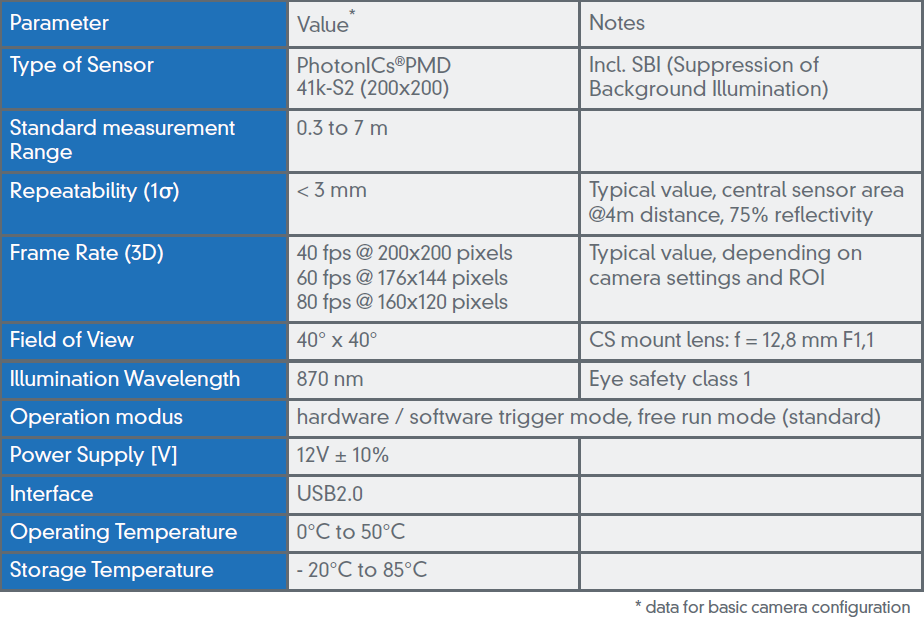
\includegraphics[scale=0.6]{Abbildungen/PMDParam}
\caption{Die grundlegende Parameter der PMD Kamera. \cite{pmde}}
\label{PMDParam}
\end{figure}

Das Hintergrundlicht, z.B. das Sonnenlicht, k�nnte die Messung der Distanz stark st�ren. Die PMD Kamera benutzt das aktive Sendersignal und einen Fremdlicht-Filter (SBI), um das Hintergrundsignal zu unterdr�cken. Au�erdem bietet die PMD Kamera die M�glichkeit, die Integrationszeit der Kamera f�r jede Messung individuell einzustellen. Die Integrationszeit bezieht sich auf die Zeitspanne, in der die Kamera zur Aufzeichnung eines Bildes dem reflektierten Licht ausgesetzt wird. F�r ein schwach reflektierendes Objekt ben�tigt der Sensor l�ngere Integrationszeit als ein stark reflektierendes Objekt, um genug Information anzusammeln. Andererseits wird aber ausreichendes Licht von hellen Objekten auf den Sensor reflektiert, wenn die Integrationszeit zu lang definiert wird. In Abbildung~\ref{PMDIntTime} wird ein Beispiel der Tiefbilder mit verschiedenen Integrationszeiten gezeigt \cite{pmdd}. 

\begin{figure}[ftb]
\centering
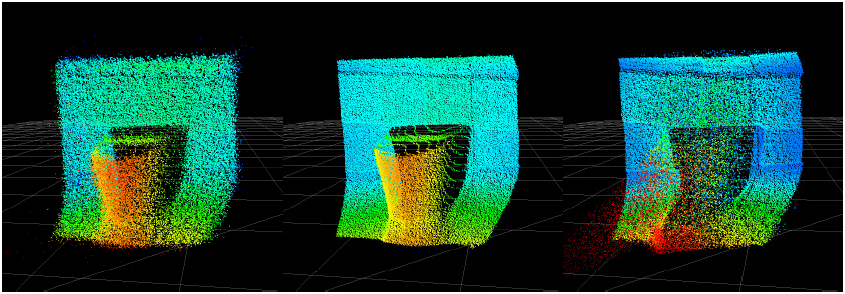
\includegraphics[scale=0.6]{Abbildungen/PMDIntTime}
\caption{Integrationszeit von 140 $\mu s$, 1400 $\mu s$ bzw. 14000 $\mu s$. Bitte beachten Sie die niedrige Signalst�rke an der linken Seite und die S�ttigung an der rechten Seite wegen der unangemessenen Integrationszeit. \cite{pmdd}}
\label{PMDIntTime}
\end{figure}

\subsubsection{Unterschied zwischen TOF Kamera und Kinect}
Kinect ist eine Hardware zur Steuerung der Videospielkonsole Xbox360, die ein sogenanntes hands-free Kontrollieren liefert, wodurch die Spieler mit einigen bestimmten Gesten oder einer kurzen Bewegung ihres K�rpers das Spiel spielen k�nnen \cite{KIN}. Um dieses Ziel zu erreichen, sammelt Kinect au�er der normalen Bildeingabe aber auch die Tiefdaten der Szene an. Wegen dieser Eigenschaft wird das Ger�t im Bereich von Computer Vision benutzt. Mithilfe des SDK ist die Programmierung der Kinect unter normalen Betriebssystemen z.B. Windows, Linux bzw. MacOS m�glich. 
\\

\begin{figure}[bft]
\centering
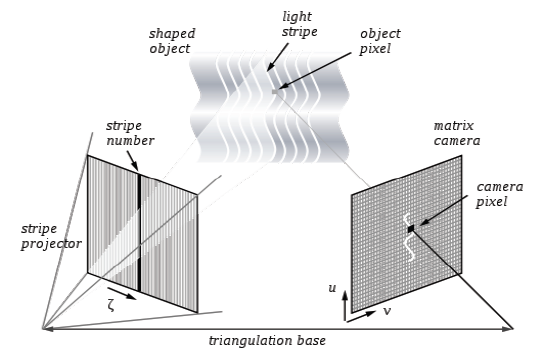
\includegraphics[scale=0.6]{Abbildungen/Kinect}
\caption{Das Arbeitsprinzip des Kinects. \cite{KINH}}
\label{Kinect}
\end{figure}

Der Unterschied zwischen TOF Kamera und Kinect k�nnen auf dem Arbeitsprinzip zur�ckgef�hrt werden. In TOF Kameras wird die Tiefdaten durch dem Laufzeitverfahren berechnet, was im \ref{TOF Kamera} erkl�rt wird. Das Abtastverfahren der Kinect hei�t Light Coding. Eine gro�e Menge von Streifen werden als Mustern auf die Szene bzw. die Objekte durch infrarotes Licht projiziert. Die ganz Szene mit diesen zus�tzlichen Mustern wird von einer infraroten Kamera des Kinects aufgenommen. Durch die Verzerrung zwischen dem vordefinierten Muster im infraroten Licht und dem von der infraroten Kamera erkannten Muster kann das Tiefbild der Szene ausgerechnet werden. Die Abbildung~\ref{Kinect} zeigt dieses Arbeitsprinzip der Kinect. Die weitere Information findet man im technischen Dokument des Firma Cadet \cite{KINH}. Der Vergleich �ber die genauen technischen Daten von PMD Kamera und Kinect wird in Tabelle~\ref{PMD and Kinect} zusammengefasst. Obwohl Kinect eine bessere Aufl�sung und gr��eres Sichtfeld hat, ist die PMD Kamera wegen ihrer hohen Bildrate und gro�en Messbereich f�r das MAROCO-System geeignet. Au�erdem mithilfe des SBI Systems ist die Arbeit der PMD Kamera unter schwieriger Umgebungsbedingung, z.B. au�erhalb des Zimmers mit starker St�rung von Sonneneinstrahlung, auch m�glich.

\begin{table}[ftb]
\begin{center}
\begin{tabular}{| l || c | c |}
\hline
Sensor & PMD CamCube & Kinect \\ \hline
Aufl�sung & 204$\times$204 Pixel & 640$\times$480 Pixel\\ \hline
Sichtfeld & $40^\circ \times 40^\circ$ & $57^\circ \times 43^\circ$ \\ \hline
Max Bildrate & 40 fps & 30 fps \\ \hline
Messbereich & 0.3 $\rightarrow$ 7.0 m & 1.2 $\rightarrow$ 3.5 m (mit Xbox Software) \\ \hline
Lange der Tiefdaten & 8 bit (unsigned char) & 11 bit \\ \hline
\end{tabular}
\caption{Die technische Daten von PMD Kamera und Kinect}
\label{PMD and Kinect}
\end{center}
\end{table}

\subsection{Daten von PMD Kamera}
Die PMD Kamera CamCube kann insgesamt 4 verschiedenen Vermessungsdaten ausgeben. Sie sind Amplitude, Intensit�t, Distanz und 3D Koordinaten. Die erste Zwei und letzte Zwei Typen der Daten k�nnen durch der Dimension in zwei Gruppen unterteilt werden. 

\subsubsection{2D Daten}
Die Intensit�t bezieht sich auf der Graustufen. Nach einer Abbildung k�nnen diese Graustufen in 0 bis 255 beschr�nkt werden, und das Ergebnis ist gleich als das Bild einer normalen Schwarz-Wei� Kamera. Die Amplitude zeigt die St�rke der Beleuchtung, die vom Objekt wegen des aktiven Sendersignal von PMD Kamera selbst gespiegelt wird. Dieser Wert kann die Qualit�t der Distanzinformation sch�tzen, d.h. das Objekt weit von Kamera liefert niedriger Amplitude als das Objekt in der N�he von der Kamera, wenn sie mit identischem Material dargestellt werden. An der Gegenseite sind die Merkmalen mit h�herem R�ckstrahlverm�gen durch Amplitudedaten einfacher betrachtet, was f�r die Erkennung der gro�en k�nstlichen Marken in unserer Arbeit sinnvoll ist.   

\subsubsection{3D Daten}
Die PMD Kamera liefert 3D Daten in zwei Formen: die reine Distanzinformation und die 3D Koordinaten. Die Distanzinformation ist die gemessene Distanz zwischen der Kamera und Objekt, was direkt durch der Formel \eqref{tof1} berechnet wird. Bez�glich diese Distanzinformation und die 2D Daten wie normale Kamera werden die 3D Koordinaten innerhalb der PMD Kamera berechnet und k�nnen durch die Schnittstelle zugegriffen werden.


\subsection{Helligkeit und S�ttigung}

\section{Markenerkennung}
Als was in Sektion \ref{mErkennung} geschrieben hat, sind viele Erkennungsalgorithmen in Open Source Library OpenCV realisiert. Der komplette Vergleich dazwischen bez�glich dem Fehlerquote, Zeitaufwand und anderen Eigenschaften wird viele gemacht, damit man dem geeigneten Algorithmus f�r seinen Bed�rfnis ausw�hlen kann. 
     
\subsection{Auswahl des Erkennungsalgorithmus}

\begin{figure}[bft]
\centering
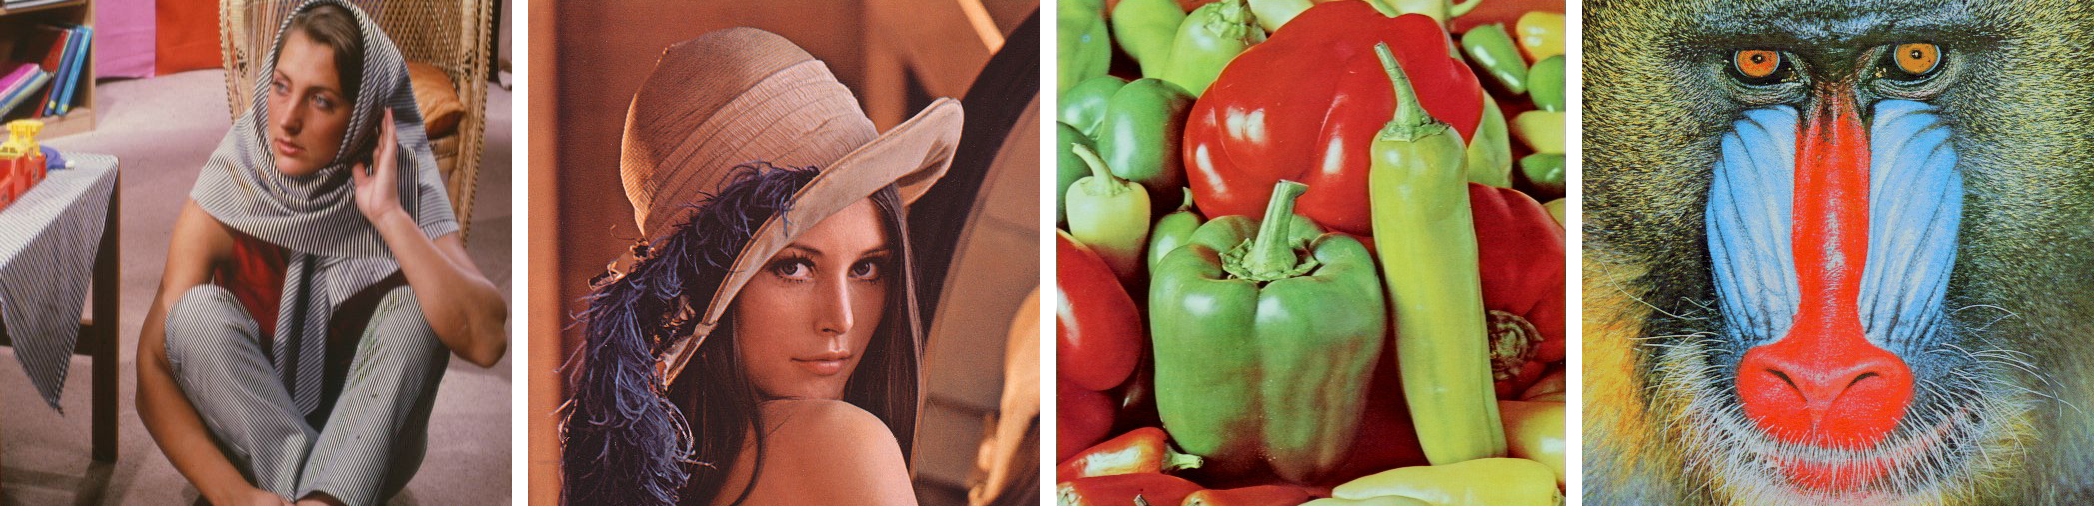
\includegraphics[scale=0.22]{Abbildungen/SampleBild}
\caption{Die vier Beispielbilder. Von link nach recht sind Barbara, Lena, Peppers und Mandril\cite{O11}}
\end{figure}

\begin{figure}[bft]
\centering
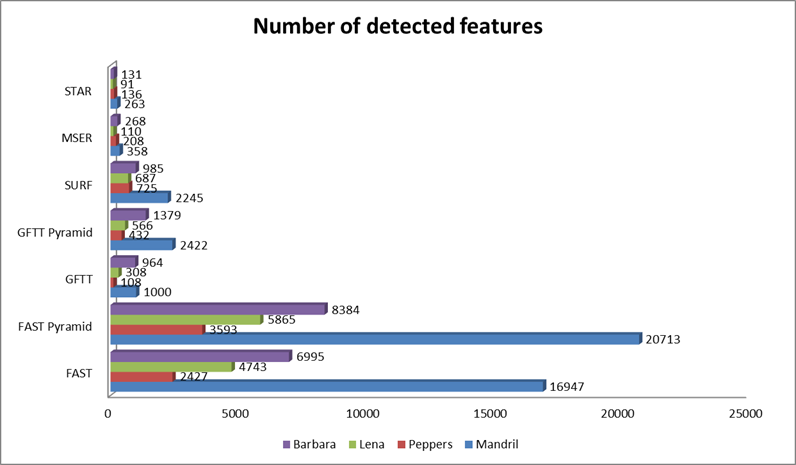
\includegraphics[scale=0.7]{Abbildungen/Number-of-detected-features}
\caption{Anzahl der erkannten Merkmalen von alle vier Beispielbildern durch verschiedene Erkennungsalgorithmen}
\label{Nodf}
\end{figure}

Odessa hat in seinem Blog einen sehr gute Vergleich f�r alle Erkennungsalgorithmen von OpenCV durchgef�hrt \cite{O11}. Vier h�ufig benutzten Beispielbilder wurden betrachtet.
\\
\\
Was besonders interessiert in seiner Arbeit ist der Vergleich �ber die Anzahl der betrachteten Punkte bzw. der durchschnittliche Fehler. Wegen des verschiedenen Prinzip zwischen der auf Ecke basierten bzw. auf Klecks basierten Algorithmen, erkennt der Algorithmus FAST viele mehr Merkmalen als SURF und STAR. Der Unterschied sieht man deutlich in der Abbildung~\ref{Nodf}. Je mehr Punkte betrachtet, desto mehr Rauchen wird im System gebracht, weil viele normalen Pixeln auch als Merkmalen erkannt werden. Das ist offensichtliche ein negativer Einfluss f�r die weitere Analyse der Daten. Abbildung~\ref{Ate} zeigt den durchschnittlichen Fehler in Pixeln von den Punktpaaren, was durch gleichem Erkennungsalgorithmus von Bezugsbilder erkannt werden. Der Algorithmus STAR erzeugt deutlich weniger Fehler in der Erkennung, und das Ergebnis h�ngt auch leicht von der Eingabe ab. Wegen der niedrigeren Fehlerquote und besserer Konzentration an gro�en Merkmalen wie Klecks ist das STAR Algorithmus f�r die Erkennung der Objekte mit k�nstlichen Marken sehr geeignet.

\begin{figure}[bft]
\centering
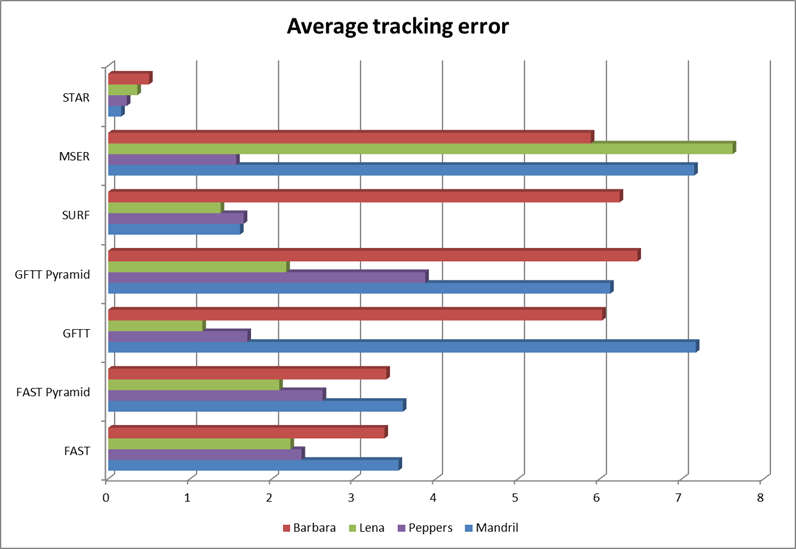
\includegraphics[scale=0.7]{Abbildungen/Average-tracking-error}
\caption{Der durchschnittliche Fehler (in Pixeln) zwischen der gegenwertigen Punkte von zwei verfolgten Bildern}
\label{Ate}
\end{figure}

\section{Markenverfolgung}

\subsection{Kalman-Filter}

\subsection{Singul�rwertzerlegung}
Sei M eine komplexe $m \times n$ Matrix mit Rang r. Dann bezeichnet die Singul�rwertzerlegung das Produkt:

\begin{equation}
M = U \Sigma V^*
\end{equation}

wobei $U$ eine Unit�re Matrix mit Gr��e $m \times m$ und $V^*$ die Adjungierte einer Unit�re Matrix mit Gr��e $n \times n$ ist. $\Sigma$ bezieht sich auf eine $m \times n$ Diagonalmatrix:

\[
\Sigma = 
\begin{pmatrix}
\sigma_1 & & & \vline & & \vdots & \\
& \ddots & & \vline & \cdots & 0 & \cdots \\
& & \sigma_r & \vline & & \vdots & \\
\hline
& \vdots & & \vline & & \vdots & \\
\cdots & 0 & \cdots & \vline & \cdots & 0 & \cdots \\
& \vdots & & \vline & & \vdots & 
\end{pmatrix}
\]

mit $\sigma_1 \geq \cdots \geq \sigma_r > 0$, wobei $\sigma_i , i=1,\ldots , r$ als die Singul�rwerte von $\Sigma$ genannt werden.
\\
\\
Mithilfe der Singul�rwertzerlegung haben Scott und Longuet-Higgins einen Algorithmus zur Bestimmung der assoziierenden Merkmale entwickelt. Seien $I$ und $J$ zwei nachfolgende Bilder und haben jeweils $m$ und $n$ Merkmale, die als $I_i (i=1,\ldots ,m)$ und $J_j (j=1,\ldots ,n$) bezeichnet werden. Dann wird eine $m \times n$ Matrix $G$ mit den Elementen

\[
G_{ij} = exp(- \frac{r_{ij}^2}{2 \sigma^2})
\]

definiert, wobei $r_{ij}$ den Abstand zwischen Merkmale $I_i$ und $J_j$ beschreibt. $\sigma$ wird als einen Standard f�r Abstand definiert, wodurch das Vergr��ern oder Verkleinern der Verschiebung des Objekts gesch�tzt werden kann. Der Wert von $G_{ij}$ nimmt durch die Erh�hung der Distanz von 1 bis 0 monoton ab. Der zweite Schritt des Algorithmus von Scott und Longuet-Higgins ist die Singul�rwertzerlegung der Matrix $G$.

\[
G = TDU
\]

wobei $T$ und $U$ die Unit�re Matrix mit jeweils Gr��e $m \times m$ und $n \times n$ sind, und $D$ eine Diagonalmatrix ist. Sei $E$ eine neue Matrix mit gleicher Gr��e von $D$, in der aber jedes diagonale Element als 1 ersetzt wird. Nach Austausch der Matrix $D$ durch Matrix $E$ erh�lt man eine neue orthogonale Matrix:

\[
P = TEU
\]

Die Aufgabe des dritten Schritts ist das Element $P_{ij}$ zu finden, was gleichzeitig das Maximum der Reihe und Spalte ist. Wenn $P_{ij}$ diese Bedingung erf�llt, sagt man, dass es eine Eins zu Eins Korrespondenz zwischen den Merkmalen $I_i$ und $J_j$ gibt. Der ganze Algorithmus kann durch folgendem Pseudocode erkl�rt werden. 

\begin{algorithm}                      % enter the algorithm environment
\caption{Bestimmung der Korrespondenz der Merkmalen von zwei Bildern}          % give the algorithm a caption
\label{alg1}                           % and a label for \ref{} commands later in the document
\begin{algorithmic}                    % enter the algorithmic environment
    \State $I,J,\sigma, Result$
    \For{$i=1 \to m$, $j=1 \to n$}
    	\State $r_{ij} \gets Dis(I_i, J_j)$
    	\State $G_{ij} \gets exp(-\frac{r_{ij}^2}{\sigma^2})$
    \EndFor
    \State $T,U \gets$ Singul�rwertzerlegung von G
    \State $E \gets m \times n$ Diagonalmatrix mit $E_{ii} = 1$
    \State $P \gets TEU$
    \For{$i=1 \to m$}
    	\State $MaxSpalteIndex[i] \gets$ Index der Spalte des maximalen Elements an Reihe $i$.
    	%\State $MaxSpalteIndex_i \gets Max$ 
    \EndFor
    \For{$i=1 \to m$}
    	\If {$P_{iMaxSpalteIndex[i]}$ ist Maximum der Spalte $MaxSpalteIndex[i]$}
    		\State $Result \gets$ Punktpaar($I_i, J_{MaxSpalteIndex[i]}$) 
    	\EndIf
    \EndFor 
\end{algorithmic}
\end{algorithm}


\section{Sch�tzung der Transformation}

\subsection{Quaternion}
%Das Quaternion
Ein Quaternion besteht aus einem Vektor mit 4 Elementen, wobei ein Element ein Skalar bezeichnet und die anderen drei eine Richtung im 3D Raum beschreiben. Quaternionen k�nnen aber auch als eine Erweiterung der komplexen Zahlen betrachtet werden, deren Imagin�rteil nach drei neuer Zahlen $i$, $j$ und $k$ entwickelt werden. Eine Normalform der Quaternion findet man im unten:

\[
q = q_0 + i q_x + j q_y + k q_z
\]

$i$, $j$ und $k$ erf�llen die sogenannte Hamilton-Regeln:

\[
i^2 = j^2 = k^2 = i j k = -1 
\]
\[
ij = k, \quad jk = i, \quad ki = j 
\]
\[
ji = -k, \quad kj = -i, \quad ik = -j
\] 

Ein andere Form mit getrennten Realteil und Imagin�rteil wird im Folgenden definiert:

\begin{equation}
\label{QForm2}
q = (q_0, \vec{q})
\end{equation}

wobei $q_0 \in \mathbb{R}$ ein Skalar und $\vec{q} \in \mathbb{R}^3$ ein Vektor ist. Sei $r$ ein andere Quaternion mit:

\[
r = r_0 + i r_x + j r_y + k r_z
\]

Analog zum Vektoren im $\mathbb{R}^4$ wird das Skalarprodukt zwischen zwei Quaternion definiert als:

\[
\langle q, r \rangle := q \cdot r := q_0 r_0 + q_x r_x + q_y r_y + q_z r_z
\]

Weiterhin kann die Quaternionmultiplikation mithilfe der Form \eqref{QForm2} berechnet als:

\begin{align}
qr & = (q_0 r_0 - \vec{q} \cdot \vec{r} , \quad q_0 \vec{r} + \vec{q} r_0 + \vec{q} \times \vec{r}) \\
\label{QMulti}
& = (q_0 r_0 - q_x r_x - q_y r_y - q_z r_z) \nonumber \\
& + i ( q_0 r_x + q_x r_0 + q_y r_z - q_z r_y ) \nonumber \\
& + j ( q_0 r_y - q_x r_x + q_y r_0 + q_z r_z ) \nonumber \\
& + k ( q_0 r_z + q_x r_y - q_y r_x + q_z r_0 )
\end{align} 

Die rechte Multiplikation von $r$ in Formel \eqref{QMulti} kann aber auch zum einen links multiplizierten Matrix umschrieben werden.

\begin{equation}
qr = 
\begin{pmatrix}
r_0 & -r_x & -r_y & -r_z \\
r_x & r_0 & r_z & -r_y \\
r_y & -r_z & r_0 & r_x \\
r_z & r_y & -r_x & r_0
\end{pmatrix}
 = \mathbf{R} q
\end{equation}

Das konjugierte Quaternion von $q$ ist definiert als:

\[
\overline{q} = q_0 - i q_x - j q_y - k q_z
\]

Das Produkt eines Quaternion und dessen Konjugierte ist eine nicht negative reelle Zahl.

\[
q \cdot \overline{q} = q_0^2 + q_x^2 + q_y^2 + q_z^2 
\]

Mithilfe des konjugierten Quaternion kann man die L�nge des Quaternion $|q|$ definieren:

\[
|q| = \sqrt{q \cdot \overline{q}}
\]

Ist die L�nge eines Quaternion gleich 1, nennt man das Quaternion ein Einheitsquaternion. F�r ein Einheitsquaternion gilt:

\[
q \cdot \overline{q} = 1 \iff \overline{q} = q^{-1}
\]

D.h. die Inverse und Konjugierte sind identisch. F�r jedes Einheitsquaternion $q \neq \pm 1$ gibt es eine entsprechende Polardarstellung:

\begin{equation}
q = \cos \alpha + \mathit{v} \cdot \sin \alpha
\label{polarQ}
\end{equation}

mit $\alpha = \arccos (q_0) \in (0,\pi)$ und $v = \frac{1}{\sin \alpha} (i q_x + j q_y + k q_z)$. 

\subsection{Beschreibung der Drehungen im Dreidimensionalen Raum mit Quaternionen}
Die Drehungen im dreidimensionalen Raum k�nnen durch die Einheitsquaternionen sehr gut beschriebt werden. Eine Abbildung der Rotation $\rho_q$ kann in folgender Form definiert werden:

\[
\rho_q : x \rightarrow q x \overline{q}
\] 

wobei $q$ ein Einheitsquaternion und $\overline{q}$ dessen Konjugierte ist. Mithilfe der Polardarstellung \eqref{polarQ} kann die Abbildung $\rho_q$ sich auf eine Drehung im $\mathbb{R}^3$ um die Achse $\mathit{v}$ mit Winkel $2\alpha \in (0, 2\pi)$ beziehen. Die entsprechende orthogonalen Matrix von $q$ ist

\begin{equation}
R =
\begin{pmatrix}
q_0^2 + q_x^2 - q_y^2 - q_z^2 & 2q_x q_y - 2q_0 q_z           & 2q_x q_z + 2q_0 q_y \\
2q_x q_y + 2q_0 q_z           & q_0^2 - q_x^2 + q_y^2 - q_z^2 & 2q_y q_z - 2q_0 q_z \\
2q_x q_z - 2q_0 q_y           & 2q_y q_z + 2q_0 q_z           & q_0^2 - q_x^2 - q_y^2 + q_z^2
\end{pmatrix}
\end{equation} 

was zur Drehgruppe SO(3) geh�rt und eine Drehung in der Matrixform repr�sentiert.

\subsection{Orientierung mit Einheitsquaternion}
Das Verfahren f�r die Orientierung der Objekte mithilfe der Quaternionen wurde erst von Horn im 1987 ver�ffentlicht \cite{H87}. Seien $D$ und $M$ zwei Punktmengen mit gleicher Gr��e $n$. Dann kann die Transformation zwischen den Punkten von zwei Menge formuliert werden als:

\begin{equation}
d_i = \mathbf{R} m_i + \mathbf{T} + e_i
\end{equation}

wobei $d_i$ und $m_i$ die i-ten Punkte der Punktmengen $D$ bzw. $M$ bezeichnen. $\mathbf{R}$ ist die Rotationsmatrix und $\mathbf{T}$ ist die Translationsmatrix. $e_i$ beschreibt den Fehler f�r die Transformation, und kann umformuliert werden als:

\begin{equation}
\label{QError}
e_i = d_i - \mathbf{R} m_i + \mathbf{T}
\end{equation}


Das Ziel des Verfahrens ist, eine Rotations- bzw. Transformationsmatrix mit minimalem Fehler zu finden, dadurch wird die Summer des Quadrats von $e_i$ betrachtet.

\begin{equation}
\sum_{i=1}^n \| e_i \|^2 = \sum_{i=1}^n \| d_i - \mathbf{R} m_i + \mathbf{T} \|^2 
\end{equation} 

Seien $\overline{d}$ und $\overline{m}$ die Schwerpunkte jeweils der Punktmenge $D$ und $M$. Dann gilt

\[
\overline{d} = \frac{1}{n} \sum_{i=1}^n d_i 
\quad \quad
\overline{m} = \frac{1}{n} \sum_{i=1}^n m_i
\]

Der Abstand von jedem Punkt zum Schwerpunkt wird berechnet als:

\[
d_i' = d_i - \overline{d}
\quad \quad
m_i' = m_i - \overline{m}
\]

und die Summe der Abst�nde erf�llt nat�rlich

\begin{equation}
\label{QDis}
\sum_{i=1}^n d_i' = 0
\quad und \quad
\sum_{i=1}^n m_i' = 0
\end{equation}

Dann kann der Fehler in Formel \eqref{QError} mit den Abst�nden zum Schwerpunkt $\overline{d}$ und $\overline{m}$ umgeschrieben werden:

\begin{equation}
e_i = d_i' - \mathbf{R} m_i' + \mathbf{T}'
\end{equation}

wobei $\mathbf{T}'$ als 

\[
\mathbf{T}' = \mathbf{T} - \overline{d} + \mathbf{R} \overline{m}
\]

definiert wird. Analog kann die Summe des Quadrats des Fehlers neu formuliert werden.

\begin{align}
\label{QError2}
\sum_{i=1}^n \| e_i \|^2 &=
\sum_{i=1}^n \| d_i' - \mathbf{R} m_i' + \mathbf{T}' \|^2 \nonumber \\
&= \sum_{i=1}^n \| d_i' - \mathbf{R} m_i' \|^2 - 2\mathbf{T}' \cdot \sum_{i=1}^n (d_i' - \mathbf{R} m_i')
+ n \| \mathbf{T}' \|^2
\end{align}

Wegen \eqref{QDis} ist der zweite Term gleich 0. Der dritte Term kann nicht negativ sein und wird 0, wenn der gesamte Fehler minimiert wird. D.h.:

\begin{align}
\label{QTran}
& \mathbf{T}' = \mathbf{T} - \overline{d} + \mathbf{R} \overline{m} = 0 \nonumber \\
\Rightarrow & \mathbf{T} = \overline{d} + \mathbf{R} \overline{m}
\end{align}

Die Formel \eqref{QTran} berechnet direkt die Transformationsmatrix durch die Rotationsmatrix und die Schwerpunkte der beiden Punktmengen. Der erste Term von \eqref{QError2} kann zu

\begin{equation}
\sum_{i=1}^n \| d_i' - \mathbf{R} m_i' \|^2 = \sum_{i=1}^n (d_i'^t d_i' + m_i'^t m_i' - 2 d_i'^t \mathbf{R} m_i')
\end{equation}

weiter formuliert werden. Dann wird die Minimierung des Fehlers durch die Bestimmung des Maximum der Summe

\begin{equation}
\sum_{i=1}^n d_i'^t \mathbf{R} m_i'
\end{equation}

erreicht. Durch Ersetzen der Rotationsmatrix mit Quaternion wird das maximierte Problem umformuliert als:

\[
\sum_{i=1}^n (q m_i'' \overline{q}) \cdot d_i''
\]

wobei $m_i'' = (0, m_{i,x}', m_{i,y}', m_{i,z}')$ und $d_i'' = (0, d_{i,x}', d_{i,y}', d_{i,z}')$ die erweiterte Quaternion f�r Punkte $m_i'$ bzw. $d_i'$ sind.
Dann gilt:

\begin{align}
\label{qmdq}
\sum_{i=1}^n (q m_i'' \overline{q}) \cdot d_i''
& = \sum_{i=1}^n (q m_i'' \overline{q}) \cdot ( d_i'' q \overline{q}) \nonumber \\
& = \sum_{i=1}^n (q m_i'') \cdot (d_i'' q)
\end{align}

Die beide Multiplikationen in Klammer k�nnen als Formel \eqref{QMulti} zum Produkt von einem Quaternion und einer Matrix umschrieben werden.

\[
q m_i'' = 
\begin{pmatrix}
0 & -m_{i,x}' & -m_{i,y}' & -m_{i,z}' \\
-m_{i,x}' & 0 & -m_{i,z}' & -m_{i,y}' \\
-m_{i,y}' & -m_{i,z}' & 0 & -m_{i,x}' \\
-m_{i,z}' & -m_{i,y}' & -m_{i,x}' & 0
\end{pmatrix}
 = \mathbf{M}_i q
\]

und 

\[
d_i'' q = 
\begin{pmatrix}
0 & -d_{i,x}' & -d_{i,y}' & -d_{i,z}' \\
d_{i,x}' & 0 & -d_{i,z}' & d_{i,y}' \\
d_{i,y}' & d_{i,z}' & 0 & -d_{i,x}' \\
d_{i,z}' & -d_{i,y}' & d_{i,x}' & 0
\end{pmatrix}
 = \mathbf{D}_i q
\]

Dann kann \eqref{qmdq} weiter ableitet werden:

\begin{align}
\label{qNq}
 \sum_{i=1}^n ( \mathbf{M}_i q) \cdot ( \mathbf{D}_i q)
 & = \sum_{i=1}^n q^t \mathbf{M}_i^t \mathbf{D}_i q \nonumber \\
 & = q^t \Big( \sum_{i=1}^n \mathbf{M}_i^t \mathbf{D}_i \Big) q \nonumber \\
 & = q^t \Big( \sum_{i=1}^n \mathbf{N}_i \Big) q \nonumber \\
 & = q^t \mathbf{N} q
\end{align}
 
wobei $\mathbf{N}_i = \mathbf{M}_i^t \mathbf{D}_i$ ist, und $\mathbf{N}$ die Summe von $\mathbf{N}_i$ beschreibt. Sei $\mathbf{H}$ die Summe der Kreuzprodukten des Punktpaars von Punktmengen $D$ und $M$.

\[
\mathbf{H} = \sum_{i=1}^n m_i d_i^t
\]

Es ist deutlich, dass die Gr��e der Matrix $\mathbf{H}$ 3 $\times$ 3 ist, deshalb kann $\mathbf{H}$ auch als

\[
\mathbf{H} = 
\begin{pmatrix}
S_{xx} & S_{xy} &S_{xz} \\
S_{yx} & S_{yy} &S_{yz} \\
S_{zx} & S_{zy} &S_{zz} 
\end{pmatrix}
\]  
  
geschrieben werden, wobei

\[
S_{xx} = \sum_{i=1}^n m_{i,x}' d_{i,x}' \quad
S_{xy} = \sum_{i=1}^n m_{i,x}' d_{i,y}' 
\]

usw. Dann kann die Matrix $\mathbf{N}$ im \eqref{qNq} durch die Elemente von $\mathbf{H}$ dargestellt werden als:

\begin{equation}
\mathbf{N} = 
\begin{pmatrix}
S_{xx} + S_{yy} + S_{zz} & S_{yz} - S_{zy} & S_{zx} - S_{xz} & S_{xy} - S_{yx} \\
S_{yz} - S_{zy} & S_{xx} - S_{yy} - S_{zz} & S_{xy} + S_{yx} & S_{zx} + S_{xz} \\
S_{zx} - S_{xz} & S_{xy} + S_{yx} & -S_{xx} + S_{yy} - S_{zz} & S_{yz} + S_{zy} \\
S_{xy} - S_{yx} & S_{zx} + S_{xz} & S_{yz} + S_{zy} & -S_{xx} - S_{yy} + S_{zz} 
\end{pmatrix}
\end{equation}

Nach dem Beweis von Horn \cite{H87} wird die Formel \eqref{qNq} Maximum, genau dann wenn $q$ der zu dem maximalen positiven Eigenwert der Matrix $\mathbf{N}$ entsprechende Eigenvektor ist. 

\section{Objekterkennung}

\subsection{DBSCAN}
DBSCAN, kurz von dem englischen Name Density-Based Spatial CLustering of Applications with Noise, ist ein auf Dichte basierter Data-Mining-Algorithmus. Die Hauptidee des Algorithmus h�ngt stark von dem Begriff ,,Dichteverbundenheit'' ab, was durch folgenden Definitionen erkl�rt wird.
\\
\\
Seien $D$ eine Punktmenge im Raum $\mathbb{R}^n$ und $Dist(p,q)$ eine darauf definierte Distanzfunktion. $\epsilon$ und MinPts sind zwei Eingaben des Algorithmus.

\begin{definition}
\textsf{$\epsilon$-Umgebung} $N_{\epsilon}(p)$ ist eine Menge der Punkte um $p$, die erf�llt
\[
N_{\epsilon}(p) = \{ q \in D | Dist(p,q) \geq \epsilon \}
\]
\end{definition}

\begin{definition}
Ein Punkt $p$ ist \textsf{direkt Dichte-erreichbar} zum Punkt $q$, g.d.w:
\begin{align*}
1) \quad & p \in N_{\epsilon}(q)  \nonumber \\
2) \quad & | N_{\epsilon}(q) | \geq MinPts \nonumber
\end{align*}
\end{definition}

\begin{definition}
Ein Punkt $p$ ist \textsf{Dichte-erreichbar} zum Punkt $q$, g.d.w es eine Kette von Punkten $p_1, \ldots , p_n$ mit $p_1 = p$ und $p_n = q$ gibt, wobei $p_{i+1}$ \textsf{direkt Dichte-erreichbar} zum $p_i$ f�r alle $i \in [1,n]$ ist.
\end{definition}

\begin{definition}
Zwei Punkte $p$ und $q$ hei�t \textsf{Dichte-verbunden}, g.d.w es ein Punkt $o$ gibt, wobei $p$ und $q$ jeweils zum $o$ \textsf{Dichte-erreichbar} sind.
\end{definition}

Mithilfe dieser Definitionen der Beziehung zwischen dem Punkten kann man jetzt eine einzige Definition des Clusters ausgeben.

\begin{definition}
Sei $C$ eine nicht leere Teilmenge von $D$. Dann hei�t $C$ ein Cluster, wenn die folgenden zwei Bedingungen erf�llt werden:
\begin{align*}
1) \quad & \text{f�r $\forall p, q \in D$, wenn $p \in C$ und $q$ ist \textsf{Dichte-erreichbar} zum $p$, dann gilt } q \in C \nonumber \\
2) \quad & \text{f�r $\forall p, q \in C$, $p$ ist \textsf{Dichte-verbunden} zum $q$} \nonumber
\end{align*}
\end{definition}

Dann k�nnen alle Punkte von $D$ in drei verschiedene Type zusammengefasst werden.

\begin{itemize}
\item Kernpunkt: Der Punkt, die Gr��e dessen $\epsilon$-Umgebung gr��er als MinPts ist.
\item Grenzpunkt: Der Punkt, dessen $\epsilon$-Umgebung nicht genug gro� ($<$MinPts), aber zu anderen Punkten Dichte-erreichbar ist.
\item Ger�usch: Der Punkt, der zu keinem Cluster geh�rt.  
\end{itemize}

\begin{figure}[ftb]
\centering
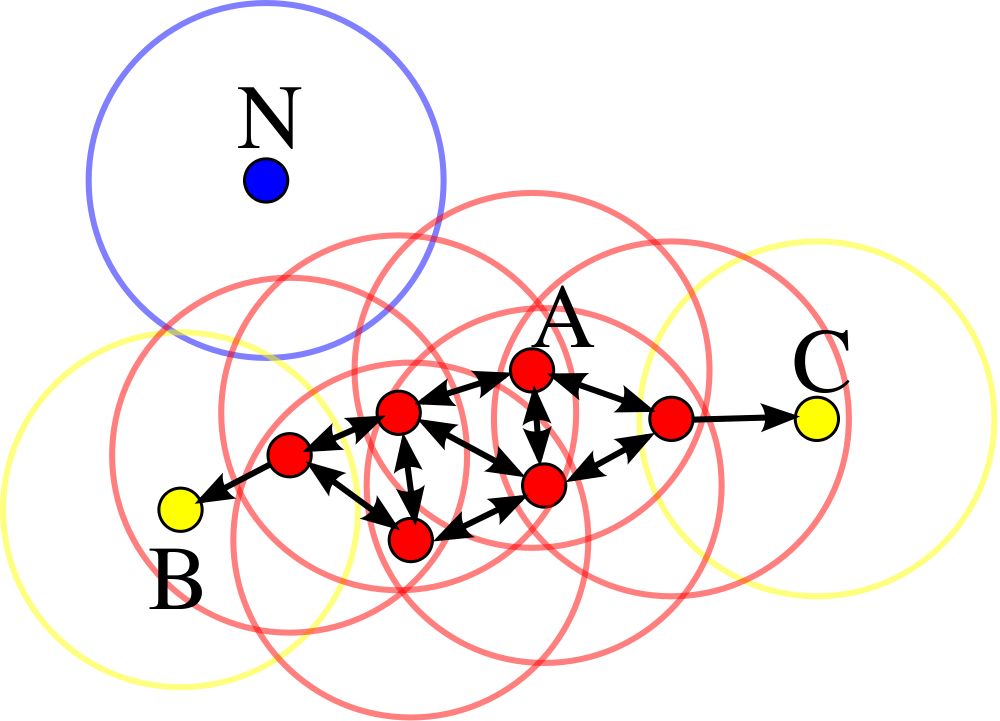
\includegraphics[scale=0.3]{Abbildungen/DBSCAN}
\caption{Ein Beispiel f�r die drei Typen der Punkte in DBSCAN-Algorithmus. Der rote Punkt A ist ein Kernpunkt. Die gelbe Punkte B und C sind die Grenzpunkte, die von roten Punkten Dichte-erreichbar sind. Wegen keine Dichte-Verbindung zwischen blau Punkt N und andere Punkte, wird N als Ger�usch erkannt. \cite{DWiki}}
\label{DBSCAN}
\end{figure}

Abbildung~\ref{DBSCAN} zeigt ein Beispiel f�r alle diesen drei Typen des Punkts, wobei die Kernpunkte mit Rot, Grenzpunkte mit Gelb und Ger�usch mit Blau beschrieben werden. Die Kreise zeigen die $\epsilon$-Umgebungen f�r die Punkte an ihrem Urspr�ngen.
\\
\\
Das Algorithmus durchl�uft f�r jeden Punkt von Punktmenge $D$ und die L�sung h�ngt von der Reihenfolge der Punkte nicht ab. Ein Kernpunkt soll zuerst gefunden werden, und dann die andere Punkte in ihrer $\epsilon$-Umgebung betrachtet werden. Zwei $\epsilon$-Umgebung werden verkn�pft, wenn sie mindesten einen identische Punkt haben. Der genaue Ablauf des DBSCAN-Algorithmus findet man unten.

\begin{algorithm}                      % enter the algorithm environment
\caption{DBSCAN}          % give the algorithm a caption
\label{algDBSCAN}                      % and a label for \ref{} commands later in the document
\begin{algorithmic}                    % enter the algorithmic environment
	\State $D, \epsilon, MinPts$
	\State Setzen $C$ zum ersten Cluster
	\For {jede $P_i \in D$}
		\If {$P_i$ ist nicht besucht}
			\State Markieren $P_i$ als besucht
			\State $N = \{ P_j \in D | Dist(P_i, P_j)<\epsilon \}$
			\If {Anzahl der Elemente von $N$ $<$ MinPts}
				\State Markieren $P_i$ als Ger�usch
			\Else
				\State F�gen $P_i$ in aktuellem Cluster $C$ ein
				\For {jede $P_j \in N$}
					\If {$P_j$ ist noch nicht besucht}
						\State Markieren $P_j$ als besucht
						\State $N' = \{ P_k \in D | Dist(P_j, P_k)<\epsilon \}$
						\If {Anzahl der Elemente von $N'$ $\geq$ MinPts}
							\State $N = N \cup N'$
						\EndIf 
					\EndIf
					\If {$P_j$ geh�rt zu keinem Cluster}
						\State F�gen $P_j$ in aktuellem Cluster $C$ ein
					\EndIf
				\EndFor
				\State Setzen $C$ zum n�chsten Cluster
			\EndIf
		\EndIf
	\EndFor
\end{algorithmic}
\end{algorithm}

\subsection{Teilgraph Isomorphismus}




\chapter{Implementierung}
\chapter{Experimentelle Auswertung}

Hier kommt die Auswertung $\ldots$

\chapter{Schlusswort}


Diese Arbeit implementiert die auf Marker basierte Objekterkennung bzw. Verfolgung im Grund auf dem Rahmenwerk MAROCO. Die Oberfl�chen der Zielobjekt werden mit retroreflektierenden Marker markiert. Eine PMD-Kamera beobachtet die ganze Szene von oben und liefert direkt die 3D-Daten. Die totale Laufzeit kann in zwei Phasen zusammengefasst werden. In der Initialisierungsphase wird die Fremdobjekt unter der Kamera gezeigt und die Marker darauf sollen herausgekannt und im System gespeichert werden. Wenn es mehr Objekte gibt, wird eine Kalibrierung am Anfang durchgef�hrt. Mills in \cite{MN00} hat eine kompakte Segmentierung der Bewegung mithilfe des sogenannten \glqq Feature Interval Graph\grqq  dargestellt. \cite{AJ05} erweitert die Arbeit von Mills. Ein auf Pyramide basiertes Clustering-Verfahren wird statt des alten auf Dreiecke basierten Clustering-Verfahren vorgeschlagen. Nach der Initialisierungsphase wird das Objekt aus dem Gesichtsfeld der Kamera verschoben. Die Erkennungsphase f�ngt genau an, wenn das gleiche Objekt wieder unter der Kamera eingebracht wird. Die reflektierende Marker sollen nochmal gesammelt werden und ein von \cite{AJ05} repr�sentierter Teilgraph-Tracker wird dann implementiert, um die Objekt zu kennen und die Position zu bestimmen.         

\cleardoublepage

% -------------------------------------------------------------------
% Anhang:
% -------------------------------------------------------------------

\appendix

\renewcommand{\baselinestretch}{1.0}

% hier die einzelnen Kapitel des Anhangs einfuegen...

%\input{MathematischeHerleitungen}

% ...
% -------------------------------------------------------------------
% Literatur:
% -------------------------------------------------------------------
\begin{thebibliography}{A}

% Konferenzbeitrag

\bibitem[Agrawal, Konolige \& Blas 2008]{AKB08}
	M.~Agrawl, K.~Konolige and M.~Blas: {\em CenSurE: Center Surround Extremas for Realtime Feature Detection and Matching}.
	\newblock in Computer Vision-ECCV 2008, pp.102-115, Springer Berlin/Heidelberg
	
\bibitem[ARToolKit]{ART}
	ARToolKit http://www.hitl.washington.edu/artoolkit/ 
	Zuletzt besucht: 02.12.2011
	
\bibitem[Arun, Huang \& Blostein 1987]{AHB87}
    K.S.~Arun, T.S.~Huang and S.D.~Blostein: {\em Least-squares fitting of two 3-D point sets}. 
    \newblock IEEE Trans Pattern Anal Machine Intell (1987) 9:698?700.
  
\bibitem[Bay et al. 2006]{B06}
	H.~Bay, A.~Ess, T.~Tuytelaars and L.V.~Gool: {SURF:Speeded Up Robust Features}.
	\newblock European Conference on Computer Vision, 2006

\bibitem[Besl \& McKay 1992]{BM92}  
    P.~Besl and N.~McKay: {\em A Method for Registration of 3-D Shapes}. 
    \newblock Trans. PAMI, Vol. 14, No. 2, 1992.
    
\bibitem[Black \& Yacoob 1997]{BY97}
    M.J.~Black and Y.~Yacoob: {\em Recognizing Facial Expressions in Image Sequences Using Local Parameterized Models of Image Motion}
    \newblock International Journal of Computer Vision 25(1), 23-48 (1997)

\bibitem[Chavarria \& Sommer 2007]{CS07}
	M.A.~Chavarria and G.~Sommer: {\em Structural ICP algorithm for pose estimation based on local features}.
	\newblock Computer Vision Theory and Applications - VISAPP , pp. 341-346, 2007

\bibitem[Chen \& Medioni 1991]{CM91}
	Y.~Chen, G.~Medioni: {\em Object Modeling by Registration of Multiple Range Images}.
	\newblock Proc. IEEE Conf. on Robotics and Automation, 1991.
	
\bibitem[Conte et al. 2004]{C04}
	D.~Conte, P.~Foggia, C.~Sansone and M.~Vento: {\em Thirty years of graph matching in pattern recognition}.
	\newblock International Journal of Pattern Recognition and Artificial Intelligence Vol. 18, No. 3 (2004) 265-298
	
\bibitem[Cordella et al. 2004]{CF04}
	L.P.~Cordella, P.~Foggia, C.~Sansone and M.~Vento: {\em A (Sub)Graph Isomorphism Algorithm for Matching Large Graphs}.
	\newblock IEEE TRANSACTIONS ON PATTERN ANALYSIS AND MACHINE INTELLIGENCE, VOL. 26, NO. 10, OCTOBER 2004
    
\bibitem[DBSCAN Wiki]{DWiki}
	DBSCAN Wikipedia: http://de.wikipedia.org/wiki/DBSCAN
	Zuletzt besucht: 11.05.2012
	
\bibitem[Dorai, Weng \& Jain 1997]{DMJ97}
	C.~Dorai, J.~Weng and A.K.~Jain: {\em Optimal registration of object views using range data}.
	\newblock IEEE Transactions on Pattern Analysis and Machine Intelligence. 19(10):1131-1137, 1997
	
\bibitem[Eggert, Lorusso \& Fisher 1997]{ELF97}
	D.W.~Eggert, A.~Lorusso, R.B.~Fisher: {\em Estimating 3-D rigid body transformations: a comparison
of four major algorithms}.
	\newblock Machine Vision and Applications (1997) 9: 272-290.
	
\bibitem[Eppstein 1999]{E99}
	D.~Eppstein: {\em Subgraph Isomorphism in Planar Graphs and Related Problems}.
	\newblock Journal of Graph Algorithms and Applications, vol. 3, no. 3, pp. 1?27 (1999)
	
\bibitem[Ester et.al 1996]{E96}
	M.~Ester, H.P.~Kriegel, J.~Sander and X.~Xu: {\em A Density-Based Algorithm for Discovering Clusters in Large Spatial Databases with Noise}.
	\newblock Knowledge Discovery and Data Mining. Seite 226-231, 1996
		
\bibitem[Haag \& Nagel 1999]{HN99}
	M.~Haag and H.~Nagel: {\em Combination of Edge Element and Optical Flow Estimates for 3D-Model-Based Vehicle Tracking in Traffic Image Sequences}.
	\newblock  International Journal of Computer Vision, Volume 35, Number 3, 295-319, 1999
	
\bibitem[Harris 1992]{H92}
	C.~Harris: {\em Tracking with Rigid Objects}. 
	\newblock MIT Press. 1992
	
\bibitem[Harris \& Stephens 1988]{HS88}
	C.~Harris and M.~Stephens: {\em A combined corner and edge detector}.
	\newblock Alvey Vision Conference, pp.147-151, 1988 
	
\bibitem[Horn \& Schunck 1981]{HS81}
	B.K.P.~Horn and B.G.~Schunck: {\em Determining optical flow}.
	\newblock Artificial Intelligence Volume 17, Issues 1?3, August 1981, Pages 185-203


\bibitem[Horn 1987]{H87}
	B.K.P.~Horn: {\em Closed-form solution of absolute orientation using unitquaternions}. 
	\newblock J. Opt. Soc. Am. A, vol. 4, 629-642, 1987. 
	
\bibitem[ICP Wiki]{IW}
	ICP Wikipedia http://de.wikipedia.org/wiki/Iterative\_ Closest\_ Point\_ Algorithm
	Zuletzt besucht: 02.02.2012
	
\bibitem[Josiger \& Kirchner 2003]{JK03}
	M.~Josiger and K.~Kirchner: {\em Moderne Clusteralgorithmen - eine vergleichende Analyse auf zweidimensionalen Daten}.
	\newblock Proc. FGML Workshop (FGML 2003), S.80-84, Karlsruhe 2003
	 
\bibitem[Jurie \& Dhome 2001]{JD01}
	F.~Jurie and M.~Dhome: {\em A simple and efficient template matching algorithm}.
	\newblock  International Conference on Computer Vision (ICCV 01) 2 (2001) 544-549.
	
\bibitem[Kinect]{KIN}
	Kinect http://www.xbox.com/en-US/kinect 
	Zuletzt besucht: 02.12.2011
	
\bibitem[Kinect-How it works]{KINH}
	Kinect-How it works
	\newblock http://www.cadet.at/wp-content/uploads/2011/02/kinect\_ tech.pdf
	Zuletzt besucht: 15.03.2012
	
\bibitem[Kanatani 1994]{K94}
	K.~Kanatani: {\em Analysis of 3-D rotation fitting}. 
	\newblock IEEE Trans Pattern Anal Machine Intell (1994) 16:543-549
	
\bibitem[Karypis et.al 1999]{K99}
	G.~Karypis, E.U.~Han and V.~Kumar: {\em CHAMELEON: A Hierarchical Clustering Algorithm Using Dynamic Modeling}.
	\newblock IEEE Computer, 32:8, S.68-75, 1999
	
\bibitem[Lamdan et al. 1988]{LSW88}
	Y.~Lamdan, J.T.~Schwatrtz and H.J.~Wolfson: {\em On recognition of 3-D objects from 2-D images}.
	\newblock In Proceedings of IEEE International Conference on Robotics and Automation, 1988

\bibitem[Lepetit \& Fua 2005]{LF05}
	V.~Lepetit and P.~Fua: {\em Monocular Model-Based 3D Tracking of Rigid Objects: A Survey}.
	\newblock Foundations and Trends in Computer Graphics and Vision Vol.1, No 1(2005) 1-89.
	
\bibitem[Lowe 2004]{L04}
	D.G.~Lowe: {\em Distinctive Image Features from Scale-Invariant Keypoints}.
	\newblock Proceedings of the International Conference on Computer Vision. 2. pp. 1150?1157, 2004 

\bibitem[Lucas \& Kanade 1981]{LK81}
	B.D.~Lucas and T.~Kanade: {\em An Iterative Image Registration Technique with an Application to Stereo Vision}.
	\newblock Proceedings of Imaging Understanding Workshop, pp. 121-130 (1981).
	
\bibitem[Messmer \& Bunke 1998]{MB98}
	B.T.~Messmer and H.~Bunke: {\em A New Algorithm for Error-Tolerant Subgraph Isomorphism Detection}.
	\newblock IEEE TRANSACTIONS ON PATTERN ANALYSIS AND MACHINE INTELLIGENCE, VOL. 20, NO. 5, MAY 1998
	
\bibitem[Mills \& Novins 2000]{MN00}
	S.~Mills and K.~Novins: {\em Motion Segmentation in Long Image Sequences}. 
	\newblock In Proceedings of the British Machine Vision Conference 2000, pp.162-171.
	
\bibitem[Odessa 2011]{O11}
	Odessa 
	\newblock http://computer-vision-talks.com/2011/01/comparison-of-the-opencvs-feature-detection-algorithms-2/ 
	Zuletzt besucht: 02.12.2011
	
\bibitem[PMD CamCube Einf�hrung]{pmde}
	PMDs CamCube Einf�hrung: http://www.pmdtec.com/fileadmin/pmdtec/downloads/documentation/datenblatt\_ camcube3.pdf
	Zuletzt besucht: 13.03.2012
	
\bibitem[PMD CamCube Entwicklungstutor]{pmdd}
	PMDs CamCube Development Tutorial: http://www.pmdtec.com/fileadmin/pmdtec/downloads/documentation/camcube\_ softwaredevelopmenttutorial.pdf
	Zuletzt besucht: 14.03.2012
	
\bibitem[Rhijn \& Mulder 2005]{AJ05}
	A.~van Rhijn and J.~D.~Mulder: {\em Optical Tracking and Calibration of Tangible Interaction Devices}.
	\newblock IPT \& EGVE Workshop, 2005.
	
\bibitem[Rosten \& Drummond 2006]{RD06}
	E.~Rosten and T.~Drummond: {\em Machine learning for high-speed corner detection}.
	\newblock European Conference on Computer Vision, vol.1, 2006
 	
\bibitem[Rusinkiewicz \& Levoy 2001]{RL01}
	S.~Rusinkiewicz and M.~Levoy: {\em Efficient Variants of the ICP Algorithm}.
	\newblock In Proceeding of the Third Intl. Conf. on 3D Digital Imaging and Modeling, pages 145-152, Quebec City, Canada

\bibitem[Scott \& Longuet-Higgins 1991]{SL91}
	G.L.~Scott and H.C.~Longuet-Higgins: {\em An algorithm for associating the features of two images}.
	\newblock In Proc. Royal Society London, 1991, vol.B244, pp.21-26.

\bibitem[Shi \& Tomasi 1994]{ST94}
	J.~Shi and C.~Tomasi: {\em Good features to track}.
	\newblock in IEEE Computer Society Conference: Computer Vision and Pattern Recognition, 1994. 

\bibitem[TOF-Kamera Wikipedia]{TOFWiki}
	TOF-Kamera Wikipedia: http://de.wikipedia.org/wiki/Time-of-flight-Sensor
	Zuletzt besucht: 02.04.2012

\bibitem[Tomasi \& Kanade]{TK91}
	C.~Tomasi and T.~Kanade: {\em Detection and Tracking of Point Features}.
	\newblock CiteSeerX - Scientific Literature Digital Library and Search Engine (United States)
	
\bibitem[Ullmann 1976]{U76}	
	J.R.~Ullmann: {\em An Algorithm for Subgraph Isomorphism}.
	\newblock Journal of the ACM (JACM), Volume 23 Issue 1, Jan. 1976 

\bibitem[Umeyama 1991]{U91}
	S.~Umeyama: {\em Least-squares estimation of transformation parameters between two point patterns}. 
	\newblock IEEE Trans Pattern Anal Machine Intell (1991) 13:376?380

\bibitem[Vaccetti, Lepetit \& Fua 2004]{VLF04}
	L.~Vacchetti, V.~Lepetit and P.~Fua: {\em Combining edge and texture information for real-time accurate 3D camera tracking}.
	\newblock Proceedings of the Third IEEE and ACM International Symposium on Mixed and Augmented Reality, 2004 
	
\bibitem[VICON]{VIC}
	http://www.vicon.com 
	Zuletzt besucht: 01.12.2011

\bibitem[Zhang et.al 1996]{Z96}
	T.~Zhang, R.~Ramakrishnan and M.~Livny: {\em BIRCH: An efficient data clustering method for very large databases}. 
	\newblock Proceedings of the 1996 ACM SIGMOD International Conference on Management of Data, Montnreal, 1996, S.103-144
	
\bibitem[Zhang \& Navab 2000]{ZN00}
	X.~Zhang and N.~Navab: {\em Tracking and pose estimation for computer assisted localization in industrial environments}. 
	\newblock Applications of Computer Vision, 2000, Fifth IEEE Workshop on.
	
\bibitem[Zhang et al. 1995]{Z95}
	Z.~Zhang, R.~Deriche, O.~Faugeras and Q.~Luong: {\em A robust technique for matching two uncalibrated images through the recovery of the unknown epipolar geometry}.
	\newblock Artificial Intelligence Volume 78, Issues 1?2, October 1995, Pages 87-119



\end{thebibliography}

\bibliographystyle{geralpha}
% -------------------------------------------------------------------
% Stichwortverzeichnis (optional)
% -------------------------------------------------------------------
%\def\indexname{Stichwortverzeichnis}
%\printindex
%\begin{thebibliography}{99}
%\bibitem{asimo} H.~Partl:
%
%\end{thebibliography}
\end{document}
